\documentclass{article}

\usepackage{graphicx} % Required for inserting images
\usepackage{float} % For figures palcement
\usepackage[a4paper, margin=2.5cm, left=2cm, right=2cm]{geometry}
\usepackage{setspace} % to change line spacing
\usepackage{eurosym} % Euro symbol
\usepackage[hidelinks]{hyperref} % for links
\usepackage{multirow} % To span table column in multiples rows
\usepackage{textcomp} % for extra symbols like registred and copyrighted
\usepackage[pdftex,dvipsnames,table]{xcolor} % for text coloring
\usepackage{svg}  % SVG images
\usepackage{subcaption} % For subcaptions
\usepackage{glossaries} % Acronyms and glossaries
\usepackage{listings}
\usepackage{color}
\usepackage{minted}
\setminted{
    linenos=true,
    autogobble,
    frame=single,
               framesep=3mm,
               xleftmargin=21pt,
               tabsize=4, fontsize=\small, breaklines
}
\newenvironment{code}{\vspace{0.5cm}\captionsetup{type=listing}}{}



% TODO text
\usepackage{xargs} % Use more than one optional parameter in a new commands
\usepackage[colorinlistoftodos,prependcaption,textsize=tiny]{todonotes}
\newcommandx{\unsure}[2][1=]{\todo[linecolor=red,backgroundcolor=red!25,bordercolor=red,#1]{#2}}
\newcommandx{\change}[2][1=]{\todo[linecolor=blue,backgroundcolor=blue!25,bordercolor=blue,#1]{#2}}
\newcommandx{\info}[2][1=]{\todo[linecolor=OliveGreen,backgroundcolor=OliveGreen!25,bordercolor=OliveGreen,#1]{#2}}
\newcommandx{\improvement}[2][1=]{\todo[linecolor=Plum,backgroundcolor=Plum!25,bordercolor=Plum,#1]{#2}}


\renewcommand{\baselinestretch}{1.5} % Line height
\setlength{\parindent}{0pt} % Remove indent
\def\arraystretch{1.3} % Change default table padding from 1 to 1.3


\title{Rapport PFE L3 - Weather Station}
\author{ZAKARIA EL KHAYDER}
\date{April 2023}

\makeglossaries

\newacronym{ap}{AP}{Access Point}
\newacronym{wifi}{WiFi}{Wireless Fidelity}
\newacronym{http}{HTTP}{Hypertext Transfer Protocol}
\newacronym{db}{DB}{Database}
\newacronym{lora}{LoRa}{Long Range - Wireless transmission technique}
\newacronym{csv}{CSV}{Comma-seperated values}

\newcounter{romancounter} % Counter to save Roman numbers count

\begin{document}

\makeatletter
\begin{titlepage}
\begin{center}
    

\includegraphics[width=7cm]{images/faculty_logo.png}
\\[1cm]
\textbf{\large{
    Faculty of Physics and Engineering \\
    University of Starsbourg 
}}

\vfill

\large{
\textbf{End of studies' project} \\[14pt]
Bachelor in Electronic Systems
}

\textbf{\large{
Weather Station: Central
}}

\vfill

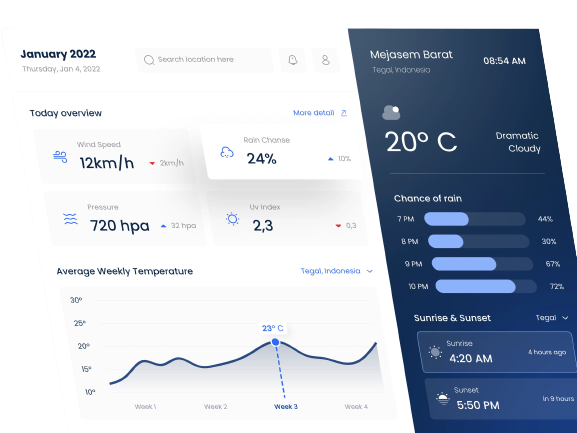
\includegraphics[width=.8\textwidth]{images/website/inspiration_bg.png}

\vfill

\textbf{Carried out by:}\\
EL KHAYDER Zakaria \\
OUFASKI Nouhaila \\
FRIES Léo

\vfill

\large{
    2022-2023
    \\[4pt]
    Made with \LaTeX
}


\end{center}
\end{titlepage}
\makeatother
\newpage

% Table of contents, figures & Tables
\pagenumbering{Roman}

\renewcommand{\contentsname}{Table of Contents} % Change title
\tableofcontents
\addcontentsline{toc}{section}{Table of Contents}
\newpage

\listoffigures
\addcontentsline{toc}{section}{List of Figures}
\listoflistings
\addcontentsline{toc}{section}{List of Listings}
\listoftables
\addcontentsline{toc}{section}{List of Tables}


\cleardoublepage
\setcounter{romancounter}{\arabic{page}} % Save counting
% Begin content
\pagenumbering{arabic}

\section{Introduction}

\subsection{Presentation}
The title of our project is: "weather station: central", which means that we will have to centralize several meteorological data acquired thanks to different sensors to a single place in which the user can use them for personal or professional use. We know that it is important to know several information about the weather in everyday life such as the temperature or the humidity level, indeed for personal use, the user may wish to know if he is beautiful in its garden in order to enjoy the outdoors, while for professional use, a company could be led to know the temperature in different rooms of its premises without wanting to go there.

\subsection{Motivation}
We decided to chose this subject for our project because it seemed to us to be something interesting to set up, requiring an electronic part using for example arduino cards, as well as a mechanical part having to protect the components from the weather.

\section{Nodes}
Our weather station's primary components are the nodes, which gather weather data through various sensors. We have selected three specific sensors: temperature, humidity, and pressure.\\
To achieve this, we have employed two Arduino Nano devices situated in different locations. Each Arduino Nano is equipped with temperature, pressure, \& humidity sensors. \\ Through LoRa communication, the collected data is transmitted to the central system, where it undergoes processing and storage for future utilization. Access to the accumulated data is facilitated through the website.


\textcolor{red}{Keep in mind:}
Our project is mainly the central part of the weather station, so this section won't go into detail as the Central section.

\subsection{Choice of parts \& material}

\subsubsection{Arduino}
For the Arduino, we don't really need anything fancy, a simple Arduino Nano will be more than sufficient.
\begin{table}[H]
    \centering
    \begin{tabular}{|l|l|}
        \hline
        \textbf{MCU} & \textbf{ATmega328P} \\ \hline
        Architecture & AVR \\ \hline
        Operating Voltage & 5V \\ \hline
        Input Voltage & 7V - 12V \\ \hline
        Clock Speed & 16 MHz \\ \hline
        Flash Memory & 32 KB (2 KB used by bootloader) \\ \hline
        SRAM & 2 KB \\ \hline
        EEPROM & 1 KB \\ \hline
        Digital IO Pins & 22 (6 PWM) \\ \hline
        Analog Input Pins & 8 \\ \hline
    \end{tabular}
    \caption{Arduino Nano Specs}
\end{table}

\subsubsection{LoRa Module}
We chose \verb|Grove - Long Range 868MHz| because of its capabilities and ease of use.
 \begin{itemize}
    \item Using RFM95 module based on SX1276 LoRa®
    \item Working Voltage: 5V/3.3V
    \item ~28mA(Avg) @+20dBm continuous transmit
    \item ~8.4mA(Avg) @standby mode
    \item ~20mA(Avg) @receive mode, BW-500kHz
    \item Working Temperature: -20 – 70℃
    \item Interface: Grove - UART (RX, TX, VCC, GND)
    \item Simple wire antenna or MHF Connector for external high gain antenna
    \item Working Frequency: 868MHz/433MHz
    \item +20dBm 100 mW Power Output Capability
    \item Size: 20*40mm
    \item Rate: 0.3kps \~ 50kps
    \item Ready-to-go Arduino libraries
    \item Reserved MHF antenna connector
\end{itemize}
\begin{table}[H]
    \caption{Grove - Long Range 868MHz Specs \& Features}
\end{table}
The module already provides an Arduino Library to interface with it through Serial communication.
\begin{figure}[H]
    \centering
    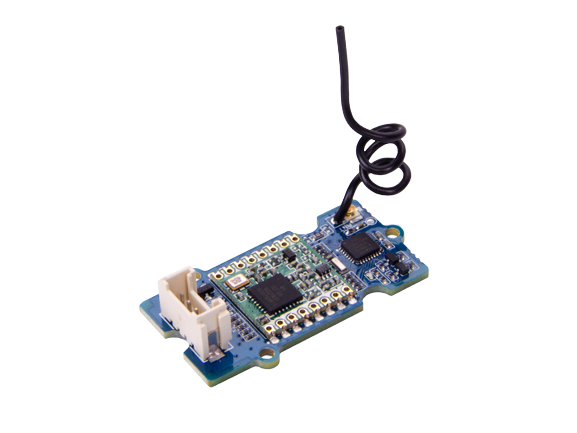
\includegraphics[width=.6\textwidth]{images/node/grove_lora.png}
    \caption{Grove - Long Range 868MHz (LoRa module)}
\end{figure}

\subsubsection{Humidity and Temperature module}
We chose \verb|DHT11| as a temperature and humidity sensor. it is cheap and very easy to interface with requiring only one data line.

\begin{itemize}
    \item Operating Voltage: 3.5V to 5.5V
    \item Operating current: 0.3mA (measuring), 60uA (standby)
    \item Output: Serial data
    \item Temperature Range: 0°C to 50°C
    \item Humidity Range: 20\% to 90\%
    \item Resolution: Temperature and Humidity both are 16-bit
    \item Accuracy: ±1°C and ±1\%
\end{itemize}
\begin{table}[H]
    \caption{DHT11 Specs \& Features}
\end{table}
\begin{figure}[H]
    \centering
    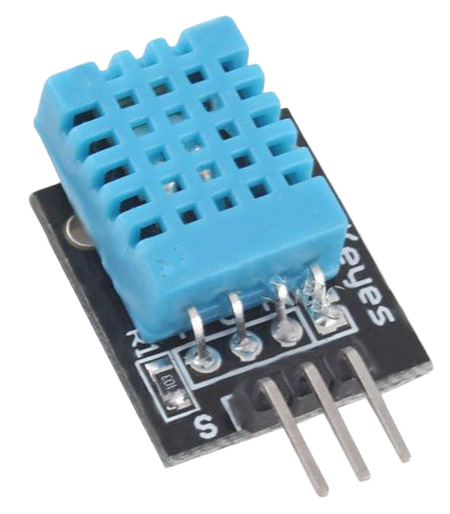
\includegraphics[width=.4\textwidth]{images/node/dht11.png}
    \caption{DHT 11}
\end{figure}

\subsubsection{Pressure Sensor}
We used \verb|BMP388| as a pressure sensor, it also measures the temperature, but we won't be using it since we already have the \verb|DHT11|.

\begin{table}[H]
    \centering
    \begin{tabular}{|p{8cm}|p{6cm}|}
        \hline
        \textbf{Parameter} & \textbf{Value} \\ \hline
        Operation range (Pressure) & 300...1250 hPa \\ \hline
        Supply voltage (VDDIO) & 1.2 V...3.6 V \\ \hline
        Supply voltage (VDD) & 1.65 V...3.6 V \\ \hline
        Interface & I²C and SPI \\ \hline
        Average typical current consumption (1 Hz data rate) & 3.4 µA @ 1Hz \\ \hline
        Absolute accuracy pressure (typ.) & P=900...1100 hPa (T=25...40°C) \& ±0.5 hPa \\ \hline
        Relative accuracy pressure (typ.) & P=900...1100 hPa (T=25...40°C) \& ±0.08 hPa \\ \hline
        Noise in pressure (lowest bandwidth, highest resolution) & 0.03 Pa \\ \hline
        Temperature coefficient offset (-20°...65°C @ 700 hPa to 1100 hPa) & ±0.75 Pa/K \\ \hline
        Long-term stability (12 months) & ±0.33 hPa \\ \hline
        Solder drift & < ±1.0 hPa \\ \hline
        Maximum sampling rate & 200 Hz \\ \hline
    \end{tabular}
    \caption{BMP388 Specs}
\end{table}
\begin{figure}[H]
    \centering
    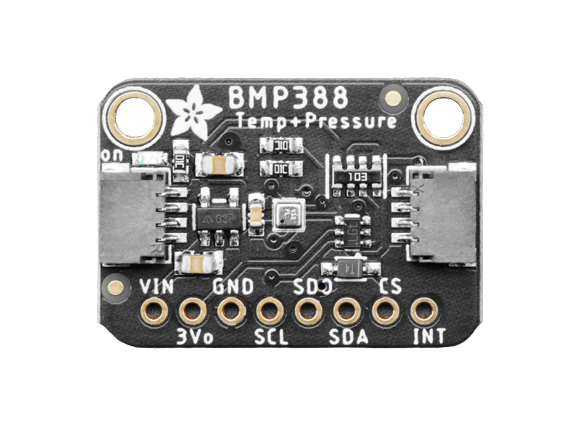
\includegraphics[width=.4\textwidth]{images/node/bmp388.png}
    \caption{DHT 11}
\end{figure}

\subsection{Electrical Schematic}
\begin{figure}[H]
    \centering
    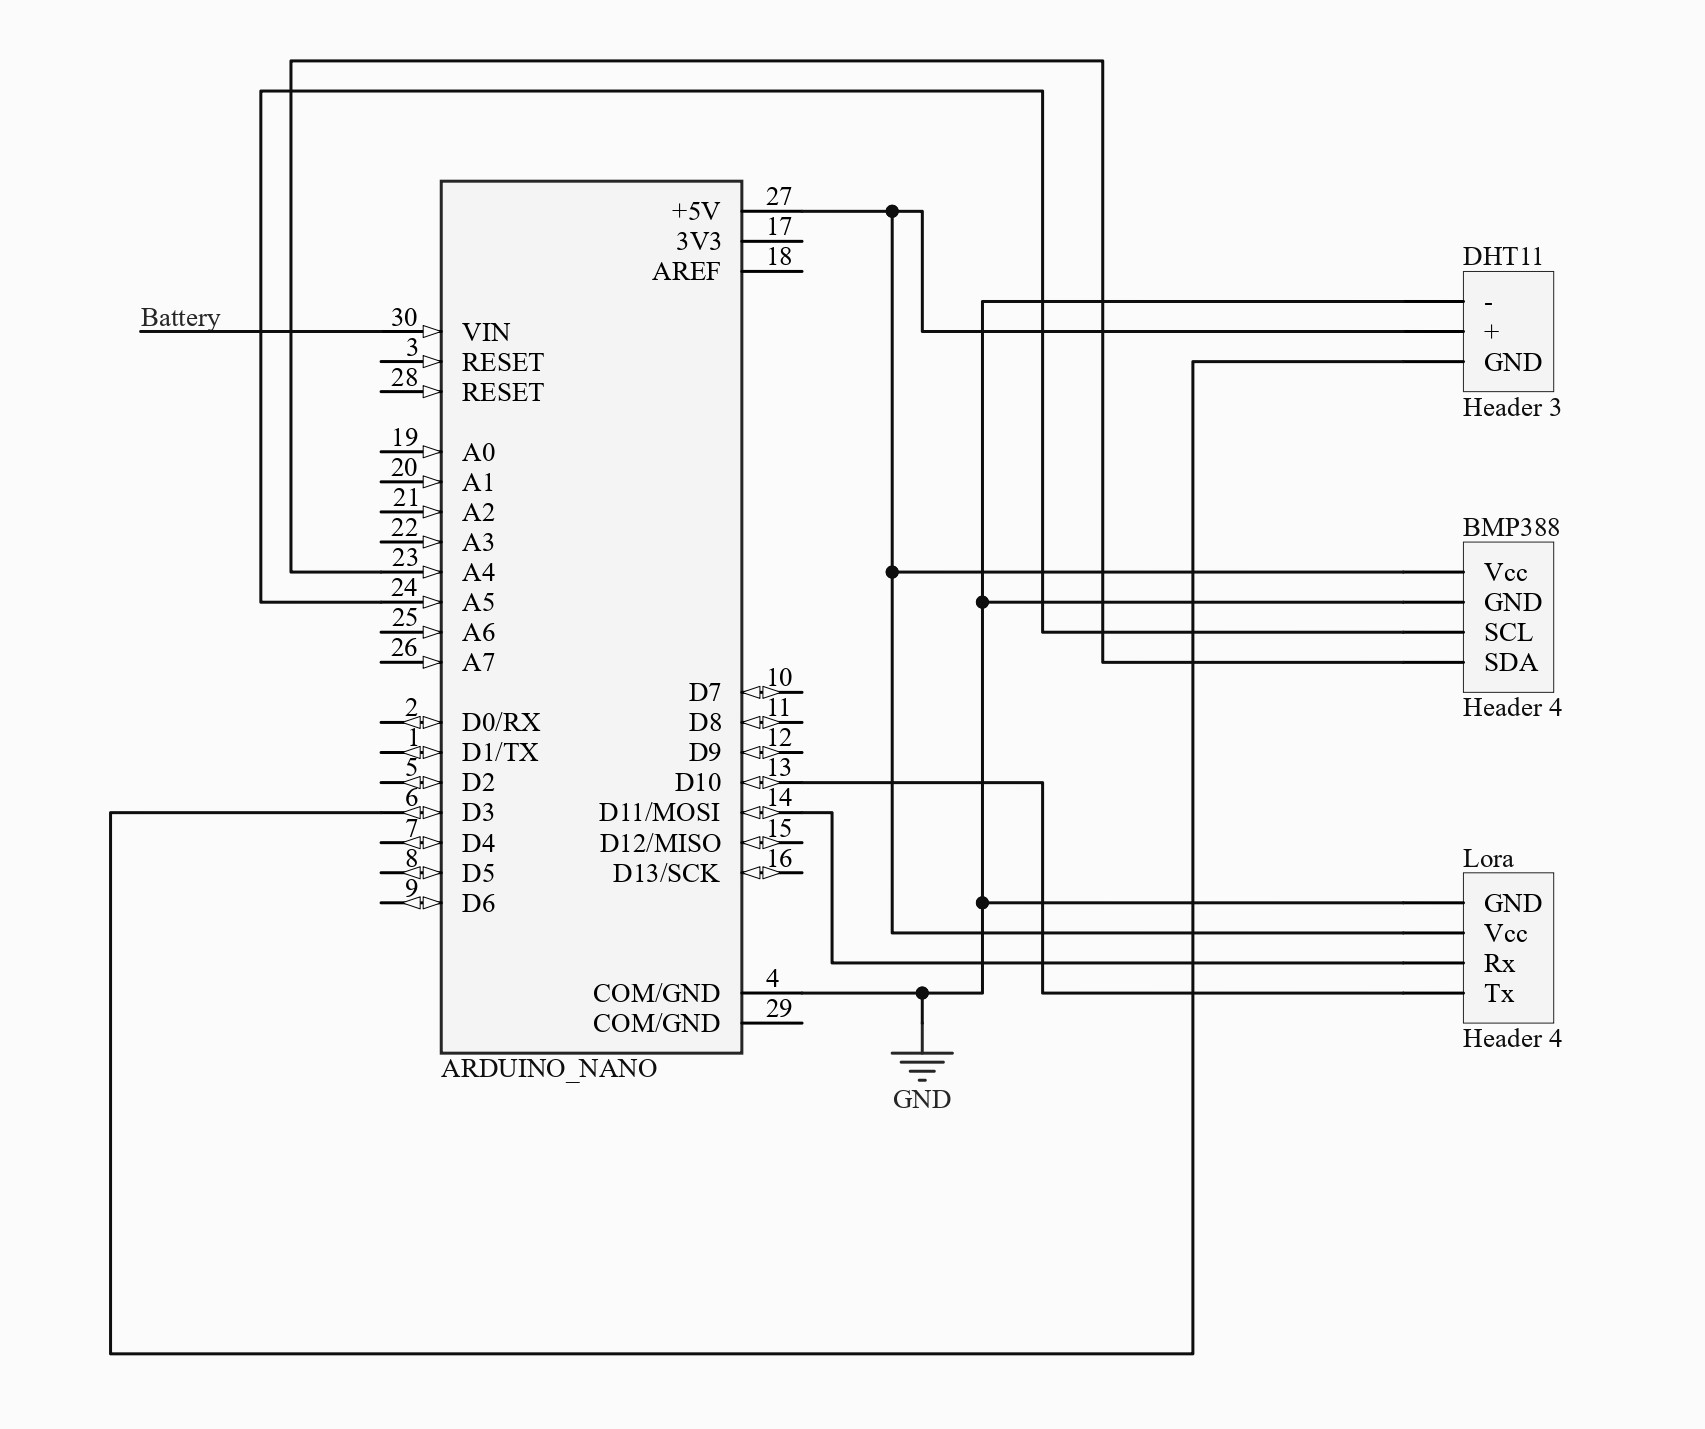
\includegraphics[width=.9\textwidth]{images/VMware Horizon_230508_235208_page-0001.jpg}
    \caption{Node Schematic}
\end{figure}

\subsection{Implementation}

\subsubsection{DHT11}
The module is very simple to interface with using Arduino \& its dedicated library. It is as simple as these for lines to initialize and fetch data.
\begin{code}
    \begin{minted}{c++}
DHT* _module = new DHT(_pin, DHT11);
_module->begin();
    \end{minted}
    \caption{DHT11 initialization}
\end{code}
\begin{code}
    \begin{minted}{c++}
float humidity = _module->readHumidity();
float temperature = _module->readTemperature();
    \end{minted}
    \caption{DHT11 interfacing}
\end{code}

\subsubsection{BMP988}
This module is a bit more verbose than its predecessor, but its library does more of the heavy lifting
\begin{code}
    \begin{minted}{c++}
DFRobot_BMP388_I2C* _module;
BMP388::BMP388()
{
    _module = new DFRobot_BMP388_I2C();
    _module->set_iic_addr(BMP3_I2C_ADDR_PRIM);
}

void BMP388::setup()
{
    Serial.println("Initializing BMP388 (Pressure Sensor)...");
    while (_module->begin() != BMP3_OK)
    {
        Serial.println("BMP388 initialization failed, Retrying...");
        delay(1000);
    }
    Serial.println("BMP388 initialized");
}

void BMP388::run()
{
    float pressure = _module->readPressure();

    float temperature = _module->readTemperature();
}
    \end{minted}
    \caption{BMP388 initiation & interfacing}
\end{code}

\subsubsection{LoRa}
\begin{code}
    \begin{minted}{c++}
Lora::Lora(uint8_t Rx, uint8_t Tx)
{
    _serial = new SoftwareSerial(Rx, Tx);
    _rf95 = new RH_RF95<SoftwareSerial>(*_serial);
}

void Lora::begin(double frequency)
{
    Serial.println("Initializing RF95 (LoRa Module)...");

    while (!_rf95->init())
    {
        Serial.println("RF95 initialization failed, Retrying...");
        delay(1000);
    }

    if (!_rf95->setFrequency(frequency))
    {
        Serial.println("RF95 frequency out of range");
        while (1)
            ;
    }

    Serial.println("RF95 initialized");
}

String Lora::_joinPayloads(String *data, size_t len)
{
    String r;

    for (int i = 0; i < len; i++)
    {
        r += data[i] + '\n';
    }

    return r;
}

bool Lora::sendPayloads(String *data, size_t len)
{
    String result = _joinPayloads(data, len);

    Serial.print("Sending ");
    Serial.print(len);
    Serial.println(" payload(s)");
    for (int i = 0; i < len; i++)
    {
        Serial.print("    ");
        Serial.println(data[i]);
    }

    uint8_t bytesBuffer[result.length()];

    result.toCharArray((char *)bytesBuffer, sizeof(bytesBuffer));

    _rf95->send(bytesBuffer, sizeof(bytesBuffer));
    _rf95->waitPacketSent();
}
    \end{minted}
\end{code}
\section{Central}
The Central is the brain and muscles of our system, I
t lives in the \textit{center} (fair enough), between the nodes and the user. It communicates with other nodes, gathers and processes data, hosts the server, and serves the web interface (HMI).\\
For this type of project, Raspberry-PI is highly recommended for such a task since it is basically a tiny computer, we can easily set up and host a Database and a server to handle \acrfull{http} requests. Unfortunately, the only available Raspi in the faculty got stolen, and due to the global chip shortage, we couldn't order another one because they were often unavailable or, if we were lucky, unbelievably expensive (at least 150 \euro).\\
Because of the above, the only option we had left was to use an Arduino for the Central. The task was already hard enough, but building it on an Arduino made it x10 harder. Nevertheless, we decided to go ahead with it, challenge ourselves, and learn something new.

\subsection{Choice of parts \& material}
\subsubsection{Arduino}
The Arduino ecosystem is a vast ocean. There are around 25 official Arduino models, making the choice of the proper Arduino harder. So before choosing one, we should determine what we need first:
\begin{itemize}
    \item \textbf{Internet Connectivity}: Ethernet is acceptable, but WiFi is preferred. This module can be external.
    \item \textbf{ROM \& SRAM}: The Central will have to execute some expensive processes, which makes RAM indispensable. ROM isn't as crucial as SRAM, we can always add external memory space if needed, which leads us to the next point.
    \item \textbf{SD Card Reader}: Sensors data should be retrievable. We can also use an external module.
\end{itemize}
After research, we decided to go with \textbf{\href{https://docs.arduino.cc/hardware/mkr-wifi-1010}{Arduino MKR WiFi 1010}}. It responds to all of our requirements.
\begin{itemize}
    \item \textbf{Internet Connectivity}: Built-in \href{https://www.u-blox.com/en/product/nina-w10-series-open-cpu}{Nina W102 uBlox module}. Compatible with WiFi 802.11b/g/n \& Dual-mode Bluetooth v4.2.
    \item \textbf{ROM \& SRAM}: With 32KB of SRAM, we believe it is more than enough to handle our internal request and process nodes' communication. And with 256KB Flash memory (ROM), we can comfortably upload our sketch without compromises.
    \item \textbf{SD Card Reader}: Unfortunately, the MKR WiFi 1010 does not have an integrated SD Card Reader, but we can easily hook up an external module as stated before. 
\end{itemize}
\textcolor{red}{Attention:} One thing to keep in our mind is that Arduino MKR WiFi 1010 works with 3.3V logic level, anything above will damage the board

\begin{table}[H]
    \centering
    \begin{tabular}{|l|l|l|}
        \hline
        \multirow{3}{*}{Board}  & Name & Arduino\textsuperscript{\tiny\textregistered} MKR WiFi 1010 \\\cline{2-3}
                                & SKU & ABX00023 \\\cline{2-3}
                                & Compatibility	& MKR \\\hline
                                
        Microcontroller & \multicolumn{2}{l|}{SAMD21 Cortex\textsuperscript{\tiny\textregistered}-M0+ 32bit low power ARM MCU} \\\hline
        
        USB connector   & \multicolumn{2}{l|}{Micro USB (USB-B)} \\\hline
        
        \multirow{6}{*}{Pins}   & Built-in LED Pin	& 6 \\\cline{2-3}
                                & Digital I/O Pins	& 8 \\\cline{2-3}
                                & Analog Input Pins	& 7 (ADC 8/10/12 bit) \\\cline{2-3}
                                & Analog Output Pins & 1 (DAC 10 bit) \\\cline{2-3}
                                & PMW Pins & 13 (0 - 8, 10, 12, A3, A4) \\\cline{2-3}
                                & External interrupts & 10 (0, 1, 4, 5, 6, 7, 8 ,9, A1, A2) \\\hline
                                
        \multirow{3}{*}{Connectivity}   & Bluetooth\textsuperscript{\tiny\textregistered} & Nina W102 uBlox module \\\cline{2-3}
                                        & Wi-Fi & Nina W102 uBlox module \\\cline{2-3}
                                        & Secure element & ATECC508A \\\hline
                                        
        \multirow{3}{*}{Communication}  & UART & Yes \\\cline{2-3}
                                        & I2C & Yes \\\cline{2-3}
                                        & SPI & Yes \\\hline

        
        \multirow{5}{*}{Power}  & I/O Voltage & 3.3V \\\cline{2-3}
                                & Input Voltage (nominal) & 5-7V \\\cline{2-3}
                                & DC Current per I/O pin & 7 mA \\\cline{2-3}
                                & Supported battery & Li-Po Single  Cell, 3.7V, 1024mAh Minimum \\\cline{2-3}
                                & Battery connector & JST PH \\\hline
                                
        \multirow{2}{*}{Clock speed}    & Processor & 48 MHz \\\cline{2-3}
                                        & RTC & 32.768 kHz \\\hline
                    
        \multirow{2}{*}{Memory} & SAMD21G18A & 256KB Flash, 32KB SRAM \\\cline{2-3}
                                & Nina W102 uBlox module & 448 KB ROM, 520KB SRAM, 2MB Flash \\\hline
                                
        \multirow{3}{*}{Dimensions} & Weight & 32 g \\\cline{2-3}
                                    & Width	& 25 mm \\\cline{2-3}
                                    & Length & 61.5 mm \\\hline
    \end{tabular}
    \caption{Arduino MKR WiFi 1010 Specs}
\end{table}

\begin{figure}[H]
    \hfill
    \begin{minipage}{.45\textwidth}
        \includesvg[width=.95\textwidth]{images/components/arduino_mkr.svg}
    \end{minipage}
    \hfill
    \begin{minipage}{.45\textwidth}
        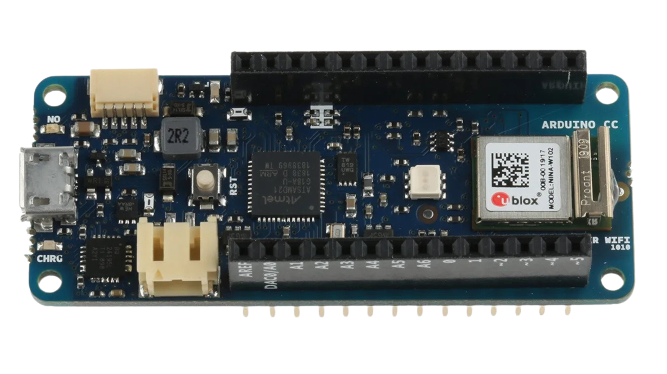
\includegraphics[width=\textwidth]{images/components/arduino_mkr.png}
    \end{minipage}
    \hfill
    \caption{Arduino MKR WiFi 1010}
\end{figure}


\subsubsection{SD Card Reader}
This one is more straightforward, we chose \href{https://digilent.com/shop/pmod-microsd-microsd-card-slot/}{Pmod MicroSD} for the simple reason of it being already available in the Faculty's inventory. Fortunately, it itself works with 3.3V logic level, which makes it compatible with Arduino MKR WiFi 1010 that we chose. In addition, it has many other impressive features:
\begin{itemize}
    \item Store and access large amounts of data from the host board
    \item No limitation on the file system or memory size of microSD card used, which is great for reasons we will discuss later
    \item 1-bit and 4-bit communication
    \item 12-pin Pmod port with \textbf{SPI interface}
\end{itemize}

\begin{figure}[H]
    \centering
    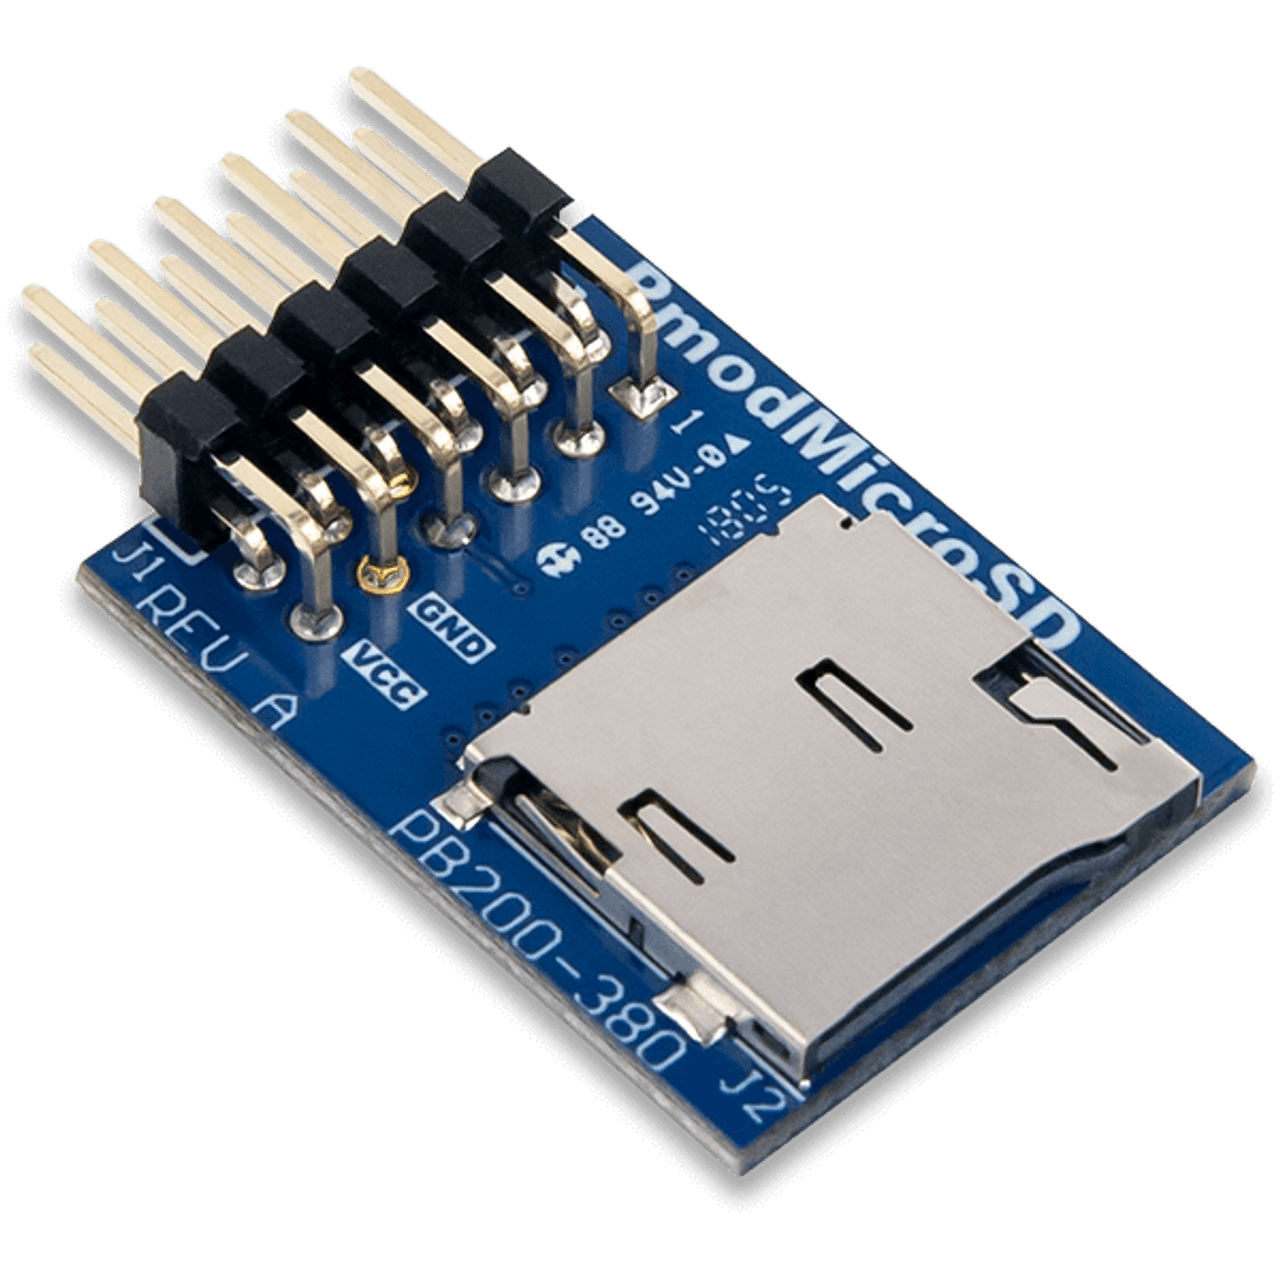
\includegraphics[height=.3\textwidth]{images/components/pmod_microsd_reader.png}
    \caption{Pmod MicroSD Reader}
\end{figure}

\subsubsection{Display}
We will be hosting the web interface on Arduino, and we will need the IP address to access the website. We can always find it out from the Router webpanel, but it would be easier for us and the user to know it without the hassle of searching for it elsewhere, here is where comes the need for a Display, besides, we can use it also to show other information such as WiFi connection Status \& LoRa signal for example. \\
We chose to use a 20x4 I$^2$C LCD Display.
\begin{itemize}
    \item Requires minimal cable connections (Only 4: Power, Ground, SDA \& SCL)
    \item Fully compatible with Arduino with numerous up-to-date libraries.
    \item Available in faculty inventory.
\end{itemize}

\begin{figure}[H]
    \centering
    \begin{subfigure}[b]{0.4\textwidth}
        \centering
        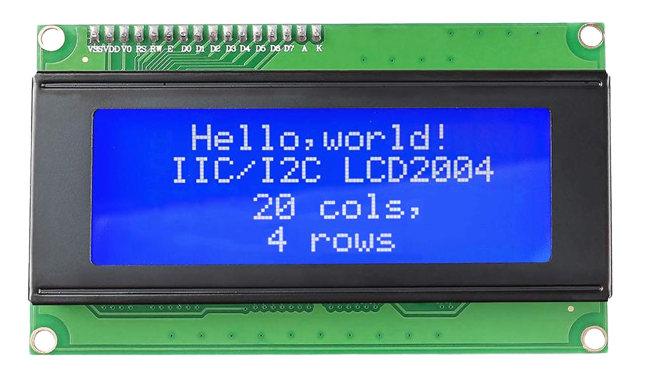
\includegraphics[width=\textwidth]{images/components/lcd_display_20x4.png}
         \caption{LCD}
    \end{subfigure}
    \hfill
    \begin{subfigure}[b]{0.49\textwidth}
        \centering
        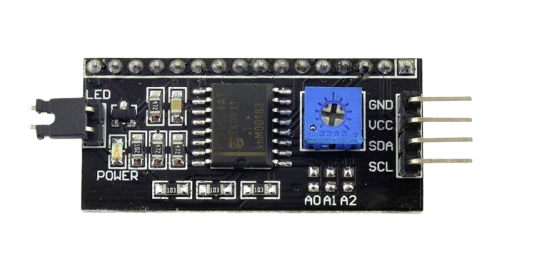
\includegraphics[width=\textwidth]{images/components/i2c_lcd_module.png}
         \caption{I$_2$C Module*}
    \end{subfigure}
    \caption{LCD Display 20x4 with I$_2$C communication module}
\end{figure}
{\footnotesize * Module usually comes pre-soldered to the LCD display}

\subsection{Architecture}
Arduino wasn't really built to be a server really, so implementing one won't be the smoothest thing to do, no doubt we will be having too many moving parts that we need to build ourselves.

\begin{itemize}
    \item \textbf{\acrshort{wifi}}: Handle \acrshort{wifi} connection \& verify connection status regularly. It should also handle any errors while connecting or that can cause a disconnection from the \acrfull{ap}
    \item \textbf{Storage}: Implement a way to easily fetch and write data to \& from the SD card. It should act like a \acrshort{db}.
    \item \textbf{Clock}: We intend to log the data received from the nodes to keep a history of previous measurements, we will need to also keep track of the time when we received those data.
    \item \textbf{\acrshort{http} handler}: Keep an eye on new \acrshort{http} connections and handle them. We will refer to this part as "server" or "application" from now on.
    \item \textbf{LCD}: Handle LCD updates, which should be triggered when data changes.
    \item \textbf{\acrshort{lora} Communication}
\end{itemize}

\textcolor{blue}{Keep in mind:} Before starting to code a project with this many moving parts, we should think about having only one source of truth, meaning that we should have only one place from where we can get information about something, for example, \acrshort{wifi} status. This concept is also known as having a \textbf{\textit{Single App Store}} or \textbf{\textit{Central App State}}. \\

\begin{figure}[H]
    \centering
    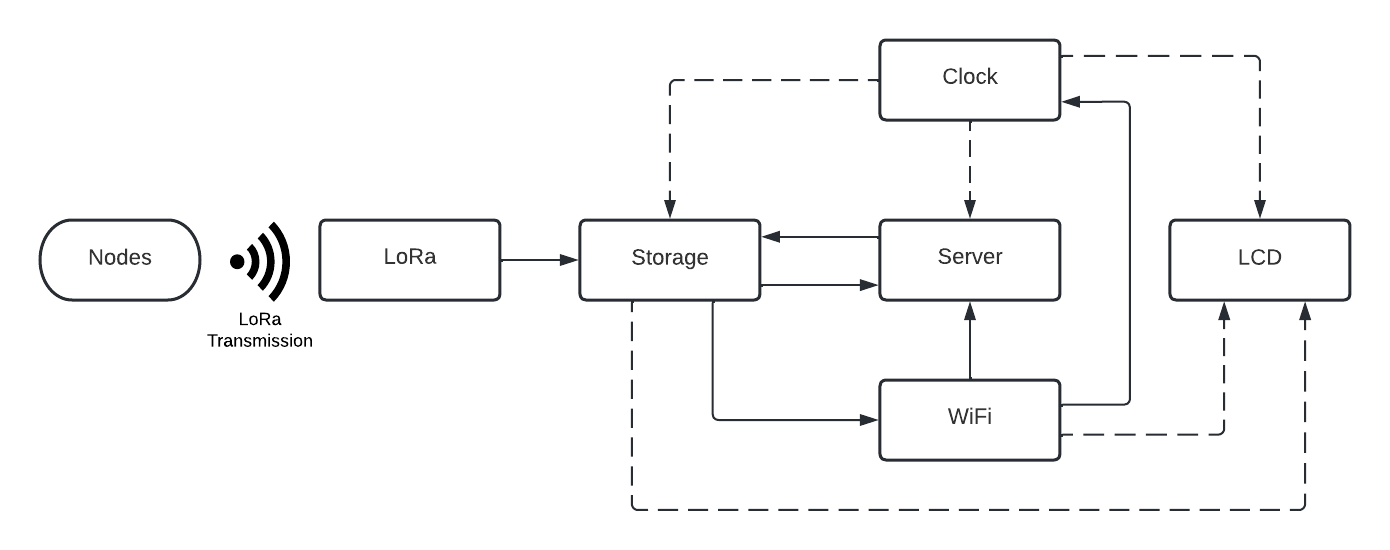
\includegraphics[width=\textwidth]{images/architecture.png}
    \caption{Central Architecture}
\end{figure}

\newcommand\dashto{\mathrel{
  -\mkern-6mu{\to}\mkern-20mu{\color{white}\bullet}\mkern12mu
}}

\textcolor{red}{Legend:}
\begin{itemize}
    \item A $\longrightarrow$ B: A affects B (Change its value).
    \item A $\dashto$ B: B reads from A.
\end{itemize}


\subsection{Implementation}

\subsubsection{WiFi}
Thanks to using MKR WiFi 1010, initiating a WiFi connection is straightforward, however, we should keep an eye on the connection status every few minutes or so in case of connection loss.
\begin{figure}[H]
    \centering
    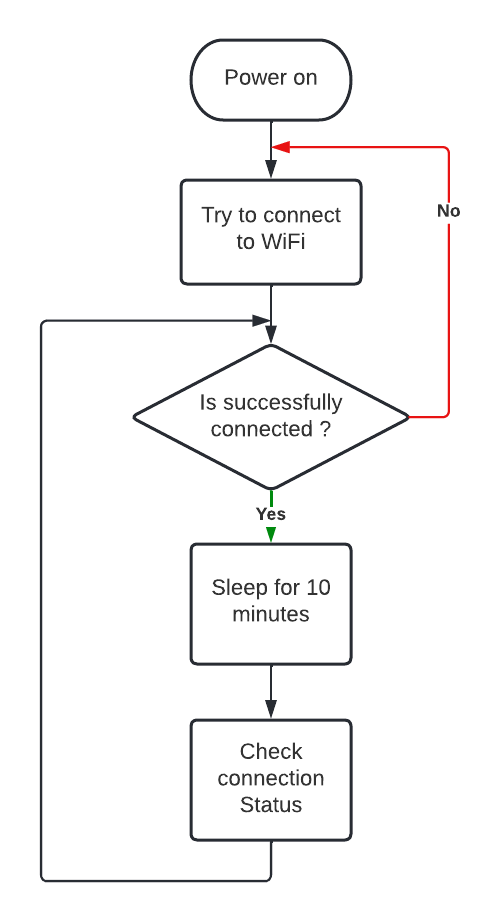
\includegraphics[width=.4\textwidth]{images/central/wifi_flowchart.png}
    \caption{WiFi implementation flowchart}
\end{figure}

\begin{code}
\caption{WiFi first connection implementation}
\begin{minted}{c++}
#include <WiFiNINA.h>

void setup() {
    if (::WiFi.status() == WL_NO_MODULE) {
    //  ^^ main namespace scope
        errHalt(F("WiFi"), F("Module not found"));
    }
    String fv = ::WiFi.firmwareVersion();
    Serial.print(F("Wifi Module detected, firmware version: "));
    Serial.println(fv);
    connect();
}
\end{minted}
\end{code}

\begin{code}
\caption{WiFi connect implementation}
\begin{minted}{c++}
void connect() {
    while (_status != WL_CONNECTED) {
        _status = ::WiFi.begin(_ssid, _password);
        delay(5000); // Wait up to 5s for connection to establish
    }
    local_ip = ::WiFi.localIP();
}
\end{minted}
\end{code}

\begin{code}
\caption{WiFi loop implementation}
\begin{minted}{c++}
void loop() {
    status = ::WiFi.status();
    if (_status != WL_CONNECTED) {
        connect();
    }
    delay(10 * 60 * 1000); // 10min
}
\end{minted}
\end{code}

This solution will work fine... until it won't! Once we will start adding other components to our systems like the storage or the server, it will brake our system because of the \verb|delay| function. \\
The \verb|delay| function is a blocking function, meaning, while it is executing, it wouldn't allow anything else to run until it finishes, so for our case, for 10min, the Arduino will be stuck in the delay function, and wasting precious time \& processing power. \\
Before going any further, we should find a way around this limitation.

\subsubsection{Poll}
\begin{figure}[H]
    \centering
    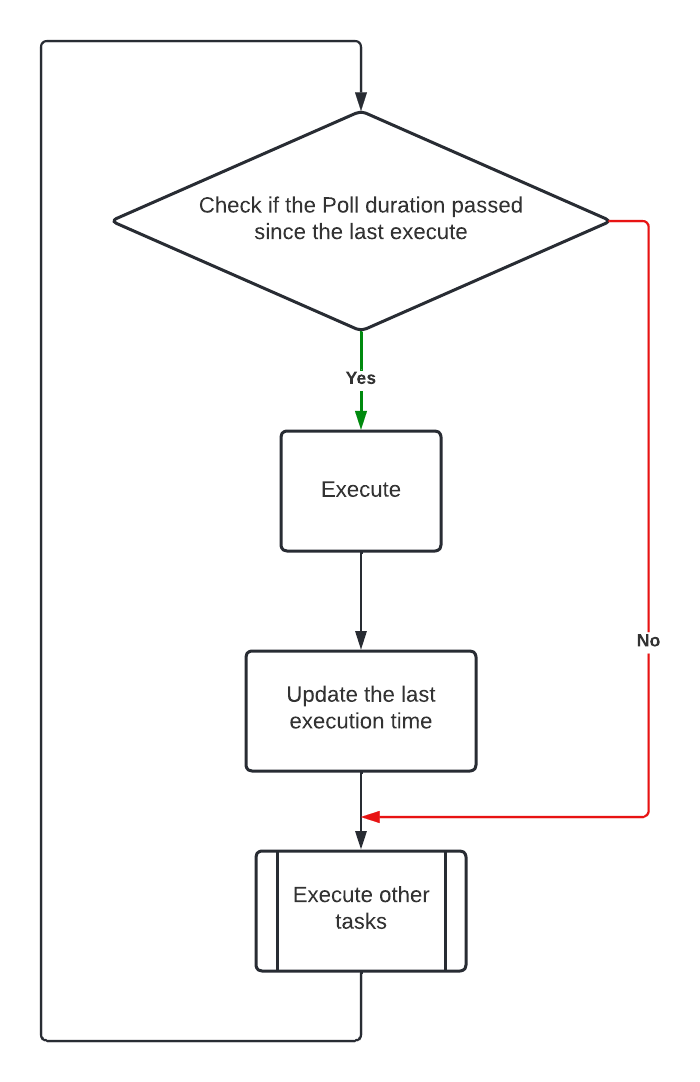
\includegraphics[width=.4\textwidth]{images/central/poll_flowchart.png}
    \caption{Poll implementation flowchart}
\end{figure}

We will be using this polling concept many times throughout our central implementation, so it is best to factor it into a C++ class. \\
We can use Arduino's \verb|millis| function to get the number of milliseconds since the program started (Arduino power on).

\begin{code}
\caption{Poll implementation}
\begin{minted}{c++}
class Poll {
    public:
        uint32_t duration;
    
        Poll(uint32_t duration) : duration(duration) {};
    
        bool shouldExecute() {
            return millis() > _last_executed_at + duration;
        }
    
        void setExecuted() {
            _last_executed_at = millis();
        }
    
    private:
        uint32_t _last_executed_at = 0; // 32bit unsigned int
};
\end{minted}
\end{code}

Now we can initiate an instance of our Poll class instead of a delay whenever we need to implement a recurring task.

\begin{code}
\caption{Poll usage example}
\begin{minted}{c++}
Poll _poll(60 * 1000); // 60_000ms = 1min
if(_poll.shouldExecute()) { <---------------------- <-
    _poll.setExecuted(); // Update execution time    ^
    // Code to execute                               ^
} // ----------------------------------------------> ^
\end{minted}
\end{code}

\subsubsection{Storage}
The storage program is very straightforward, we should only initiate the SD module connection on the Arduino's startup, however, there are some limitation that we should be aware of that concerns the FAT32 filesystem, which is the only filesystem supported by the default Arduino SD library. \\
\begin{table}[H]
    \centering
    \begin{tabular}{|l|p{9cm}|p{5cm}|}
    \hline
    Filesystem & Max. Path Length & Max. Filename Length \\
    \hline
    (*) Btrfs & No limit defined & 255 bytes \\
    \hline
    (*) ext2 & No limit defined & 255 bytes \\
    \hline
    (*) ext3 & No limit defined & 255 bytes \\
    \hline
    (*) ext4 & No limit defined & 255 bytes \\
    \hline
    (*) XFS & No limit defined & 255 bytes \\
    \hline
    (*) ZFS & No limit defined & 255 bytes \\
    \hline
    APFS & Unknown (**) & 255 UTF-8 characters \\
    \hline
    \rowcolor{red!25} FAT32 & 32,760 Unicode characters with each path component no more than 255 characters & 8.3 (255 UCS-2 code units with VFAT LFNs) \\
    \hline
    exFAT & 32,760 Unicode characters with each path component no more than 255 characters & 255 UTF-16 characters \\
    \hline
    NTFS & 32,767 Unicode characters with each path component (directory or filename) up to 255 characters long (MAX\_PATH) & 255 characters \\
    \hline
    \end{tabular}
    \caption{Path and Filename Length Limitations for different file systems}
\end{table}
{\footnotesize * In Unix environments, PATH\_MAX with 4096 bytes and NAME\_MAX with 255 bytes are very common limitations for applications including the Shell. \\
** Although not officially documented, when searching on the internet there is a limit with path names exceeding 1024 bytes. Users report warnings in Finder, the Shell, or apps about this behavior. }\\


As stated by the above table, FAT32 has a very strict limit on the file name, where it can only have 8 characters maximum for the name and 3 others for the file extension.\\
That already makes it hard for us since the default HTML file extension length is 4 characters (.html), we will also have a problem if we need to ever include an image file such as a JPEG (.jpeg) or something else, let alone the filenames which are limited to 8 characters maximum. \\

We could try to find a way around these limitations with some fancy tricks, but  as the French proverb says: "Chercher midi à quatorze heures". \\

We can use a 3rd party Arduino library \verb|SdFat.h| to do the heavy lifting for us. The usage is almost identical for the default Arduino one, except that for this library, we need to define a global variable to access the storage.

\begin{code}
    \begin{minted}{c++}
SdFat sd;

void setup() {
    if (!sd.begin(SdSpiConfig(SD_CS_PIN, DEDICATED_SPI, SD_SCK_MHZ(50)))) {
        // Throw an error and halt the program
        errHalt(F("SD card"), F("Initialisation failed!")); 
    }
    Serial.println(F("SD Card initialized successfully!"));
}
    \end{minted}
    \caption{SD card reader initialization}
\end{code}

For now, that is all that we need for the storage. Each time we need to read a file from the SD card, we can use the already initiated \verb|sd| variable.

\subsubsection{Clock}
We will use \href{www.worldtimeapi.org}{worldtimeapi.com}'s free API to get the current Unix time. This step should be executed only after already initializing the WiFi connection. \\
The API returns either a JSON or simple text response, we can get the JSON and parse it the same way we used to parse payloads in our nodes using \verb|ArduinoJSON.h| library.\\
We can also add a timer to refresh the time every 24 hours for example. this step is not really needed since Arduino can already keep a relatively precise time, but it won't hurt to add this step. 
\begin{figure}[H]
    \centering
    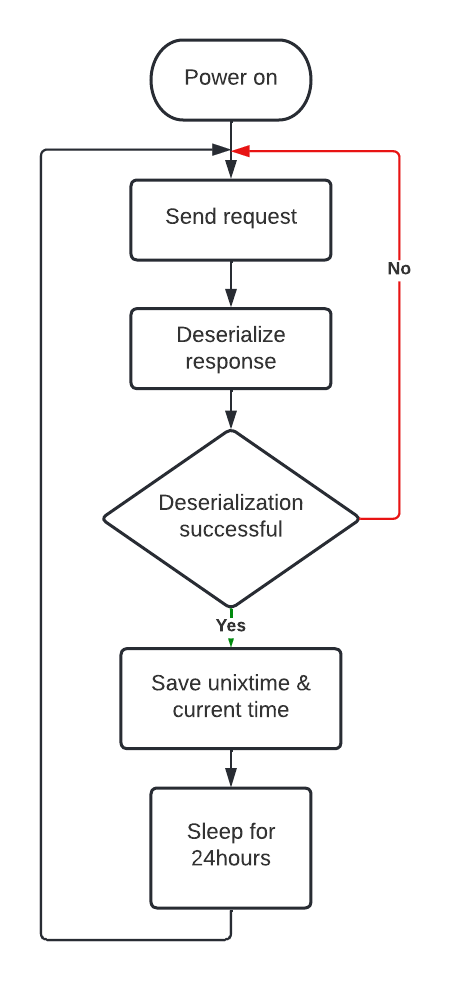
\includegraphics[width=.4\textwidth]{images/central/clock_flowchart.png}
    \caption{Clock implementation flowchart}
\end{figure}

Now getting the current Unix time at any moment is as simple as this simple equation
$$
t_{now} = t_{UnixTime} + \frac{millis() - t_{FetchedAt}}{1000}
$$
We should divide by 1000 to convert from milliseconds to seconds. \\
We can encapsulate this code in a single function for ease of use. \\
\begin{code}
\caption{Clock time fetching implementation}
\begin{minted}{c++}
uint32_t _unix_timestamp = 0;
const String _HOST_NAME = F("www.worldtimeapi.org");
const String _PATH_NAME = F("/api/timezone/Europe/Paris");
Poll _fetch_poll(24 * 60 * 60 * 1000); // 24 hours
WiFiClient _wifi = WiFiClient();
HttpClient _client = HttpClient(_wifi, _HOST_NAME);
uint32_t _fetched_at = 0;

void fetch() {
    DynamicJsonDocument json(1024);
    _client.get(_PATH_NAME);
    int statusCode = _client.responseStatusCode();
    if (statusCode < 200 || statusCode >= 300) return;
    String response = _client.responseBody();
    _client.stop();
    DeserializationError error = deserializeJson(json, response.c_str());
    if (error) return;
    _unix_timestamp = json["unixtime"];
     _fetched_at = millis();
    _fetch_poll.setExecuted();
}

uint32_t time()  {
    return _unix_timestamp + (millis() - _fetched_at) / 1000;
}
\end{minted}
\end{code}

\subsubsection{LoRa}
We already implemented the LoRa module initialization code in the nodes section. However, we should implement two functions for receiving and parsing the payloads.

\begin{figure}[H]
    \centering
    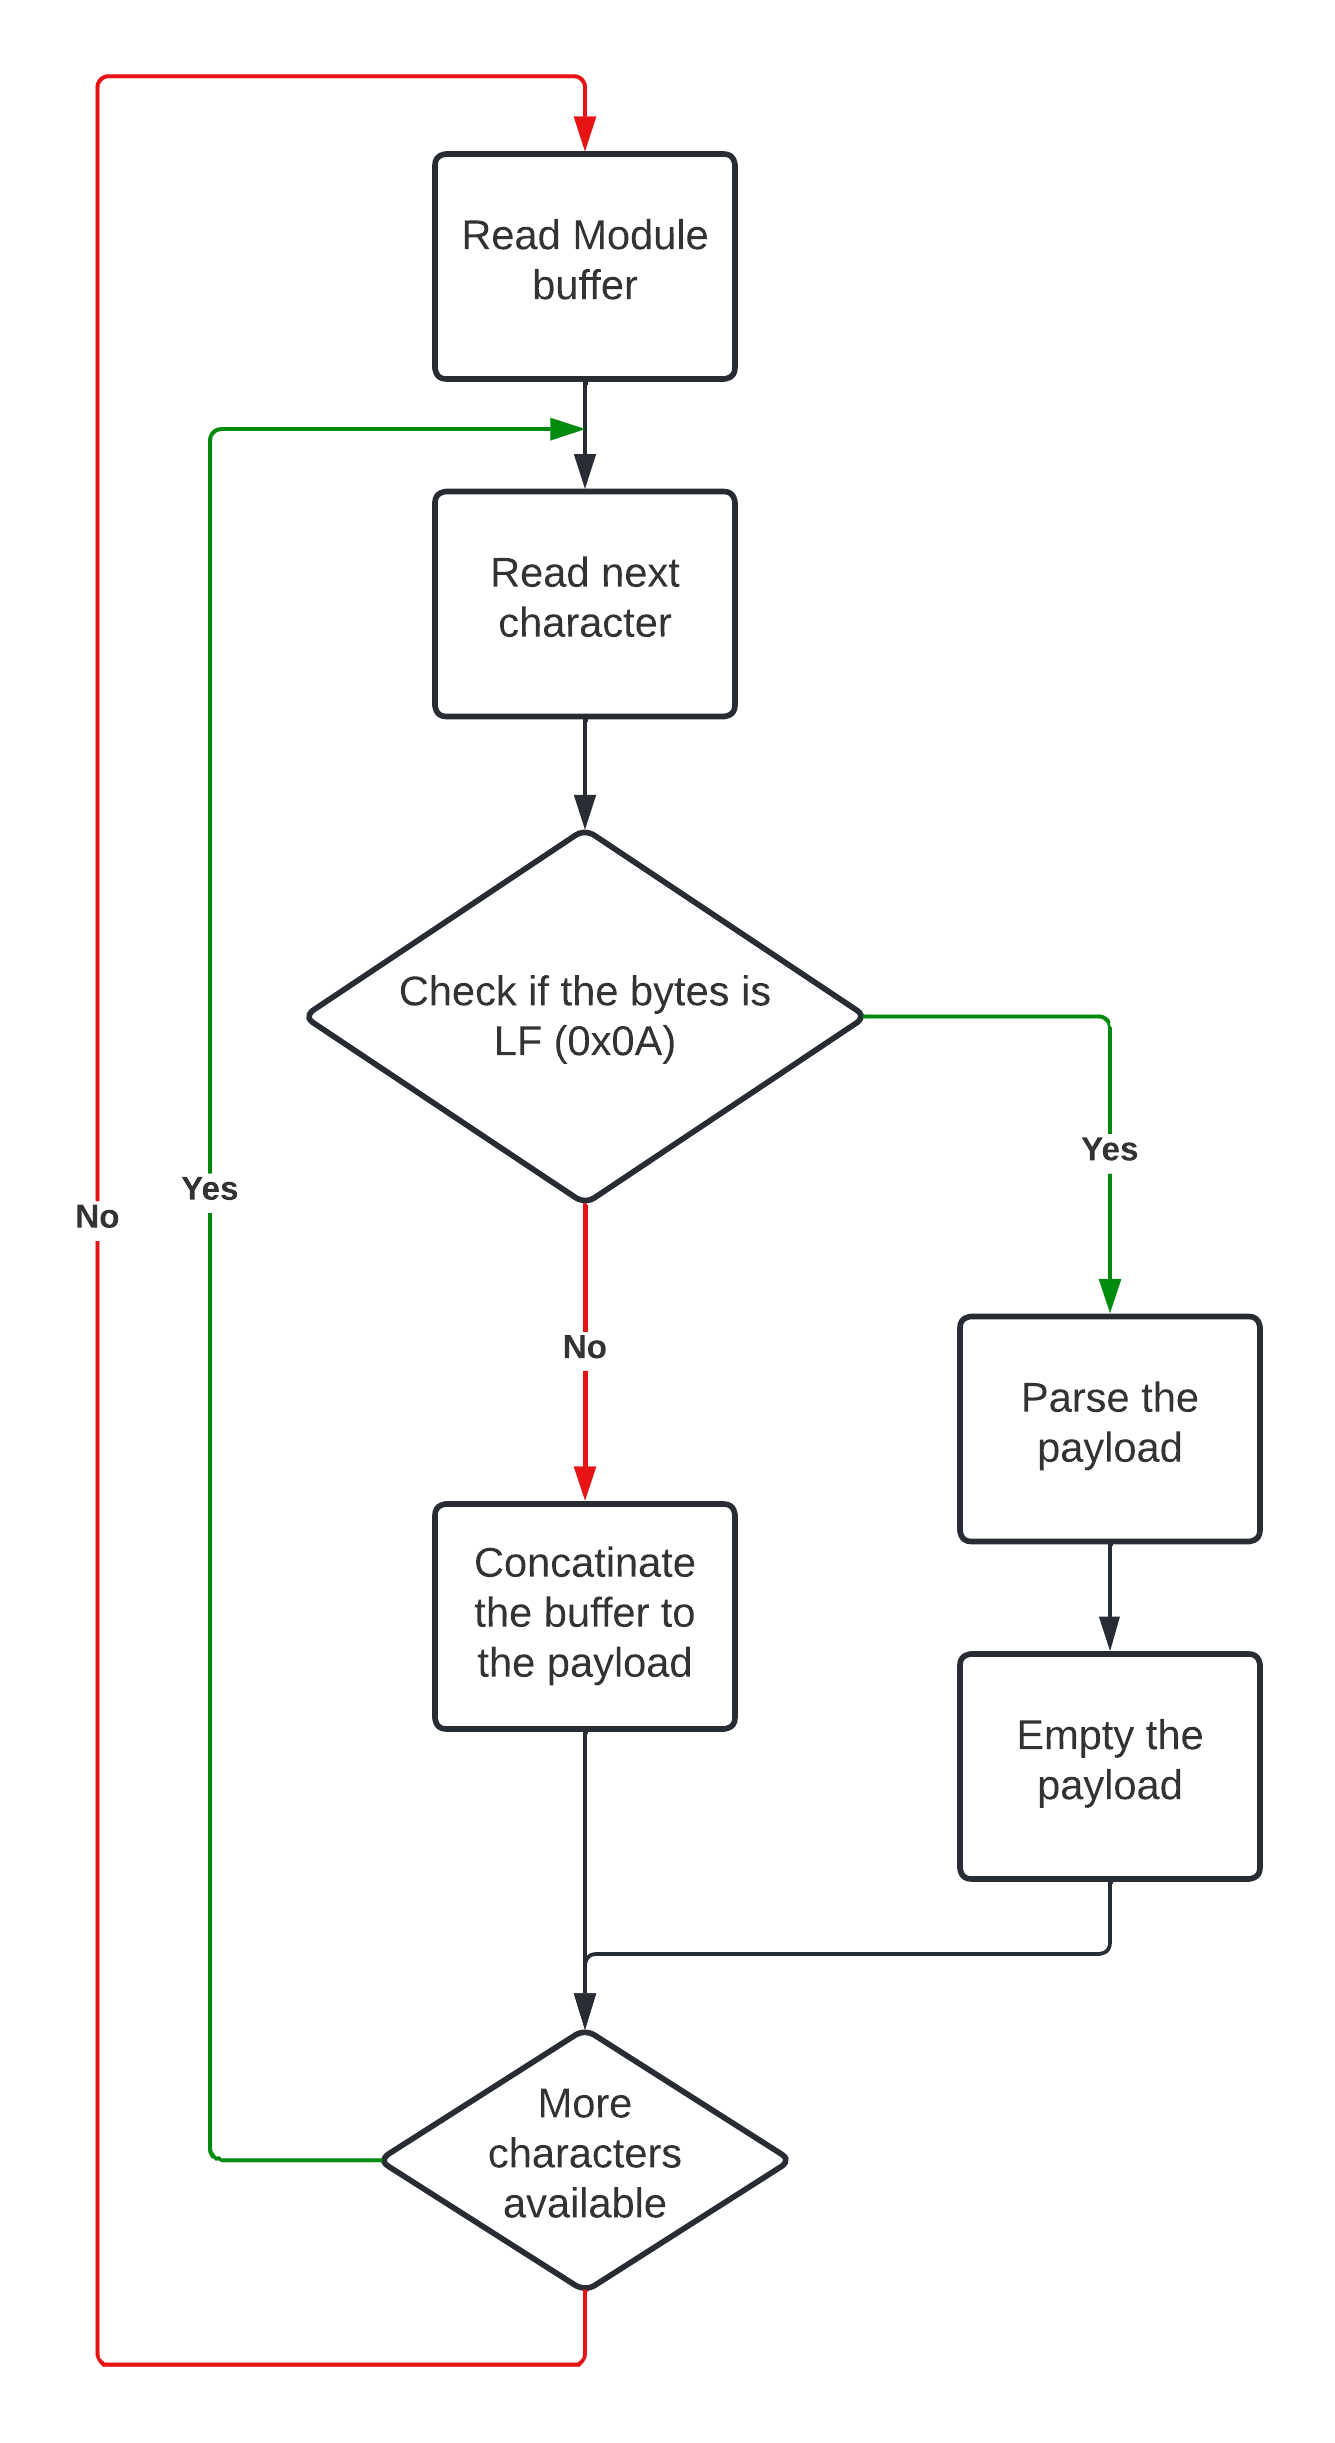
\includegraphics[width=.5\textwidth]{images/central/lora_read_flowchart.png}
    \caption{LoRa payload read flowchart}
\end{figure}

\begin{code}
\begin{minted}{c++}
void loop() {
    if (rf95.available()) {
        char buf[RH_RF95_MAX_MESSAGE_LEN];
        uint8_t len = sizeof(buf); // Equal to RH_RF95_MAX_MESSAGE_LEN
        if (!rf95.recv((uint8_t *)buf, &len)) {
            Serial.println("LoRa receive failed");
            return;
        }
        for (size_t i = 0; i < len; i++) {
            if (buf[i] == '\n') {
                parsePayload();
                buffer = "";
            } else {
                buffer += buf[i];
            }
        }
    }
}
\end{minted}
\end{code}

Payload parsing is straightforward, we should only deserialize the JSON data, and save it to the db file with the current Unix time as a \acrfull{csv} entry.

\begin{code}
\caption{LoRa payload parse implementation}
\begin{minted}{c++}
void parsePayload() {
    DynamicJsonDocument doc(512);
    DeserializationError error = deserializeJson(doc, buffer);
    if (error) return;
    const char *node = doc["node"];
    const char *measure = doc["measure"];
    double value = doc["value"];
    File db = Storage::sd.open("db.csv", FILE_WRITE);
    if (!db)
        errHalt(F("SD Card"), F("DB file open failed"))
    db.print(node);
    db.print(",");
    db.print(measure);
    db.print(",");
    db.print(value);
    db.print(",");
    db.println(Clock::time());
    db.close();
}
\end{minted}
\end{code}

\subsubsection{Server}
Now that we implemented everything, we can jump on to implementing the actual HTTP server. \\
For the sake of not having to parse the verbose HTTP protocol request ourselves, we will be using an external library that will do the heavy lifting for us: \verb|aWOT.h|.\\
The library is easy to use, we should just initialize it once by registering allowed routes and their handlers on startup and then we can pass HTTPServer requests to it to process.

\begin{code}
\caption{Server}
\begin{minted}{c++}
void setup() {
    _server.begin();
    _app.get("/api/db", &RequestHandlers::db);
    _app.get(&RequestHandlers::staticFiles);
}

void loop() {
    WiFiClient client = _server.available();
    if (client.available()) {
        _app.process(&client);
        client.stop(); //  Force disconnect to free the queue
    }
}
\end{minted}
\caption{Server setup and loop implementations}
\end{code}

We register three handlers:
\begin{itemize}
    \item \textbf{/api/db}: This route will return the db file content
    \item \textbf{Static files (website)}: Should look through the storage, if the file exists it should return its content
\end{itemize}

\begin{code}
\begin{minted}{c++}
namespace RequestHandlers {
    void staticFiles(Request &req, Response &res) {
        if (strlen(req.path()) == 1) {
            return file(req, res, "/index.html");
        }
        return file(req, res, req.path());
    }

    void db(Request &req, Response &res) {
        File file = Storage::sd.open("db.csv");
        if (!file)
            return;
        while (file.available())
            res.write(file.read());
        file.close();
        res.end();
    }

    void file(Request &req, Response &res, const char *filename) {
        String filepath = Server::STATIC_FOLDER + filename;
        if (!Storage::sd.exists(filepath)) {
            res.sendStatus(404);
            return;
        }
        File file = Storage::sd.open(filepath);
        if (file.isDirectory()) {
             res.sendStatus(403);
            return;
        }
        const String *contentType = Server::fileContentType(&filepath);
        if (contentType != NULL)
            res.set("Content-Type", contentType->c_str());
        while (file.available())
            res.write(file.read());
        res.end();
        file.close();
        return;
    }
}     
\end{minted}
\caption{Server requests handlers implementation}
\end{code}

\subsubsection{Main .ino file}
After implementing all the above, we need to call each of these functions in our main Arduino .ino file.

\begin{code}
\begin{minted}{c++}
#include "src/WiFi.h"
#include "src/Server.h"
#include "src/Clock.h"
#include "src/Storage.h"
#include "src/LCD.h"
#include "src/Lora.h"

const char *WiFi::_ssid = "TestNetwork";
const char *WiFi::_password = "00000000";

void setup()
{
    Serial.begin(115200);
    LCD::setup();
    Storage::setup();
    Lora::setup();
    WiFi::setup();
    Server::setup();
    Clock::fetch();
}

void loop() {
    WiFi::loop();
    Server::loop();
    Clock::loop();
    Lora::loop();
}
\end{minted}
\caption{Main .ino file implementation}
\end{code}


That was the last part we had to implement in our server, we now should just copy the website files into the static folder on our SD card and insert it into the SD card Reader. 
\section{Website}
In this section, we will not be providing any piece of code because of the verbose nature of web coding (Especially CSS). \\
All of the source code can be found in the Seafile folder dedicated to this project.

\subsection{Used Technologies}
\begin{itemize}
    \item HTML: to build the website skeleton
    \item Tailwind CSS: used instead of css to avoid \verb|CSS hell|
    \item Typescript: used instead of Javascript to write a safer code that won't fail on runtime
    \item Vue.js: used as frontend library to make reactivity easier
\end{itemize}


\subsection{Design}
We took inspiration from a \href{www.dribbble.com}{Dribbble.com} design of \href{https://dribbble.com/syahrulfalah}{Syahrul Falah}.

\begin{figure}[H]
    \centering
    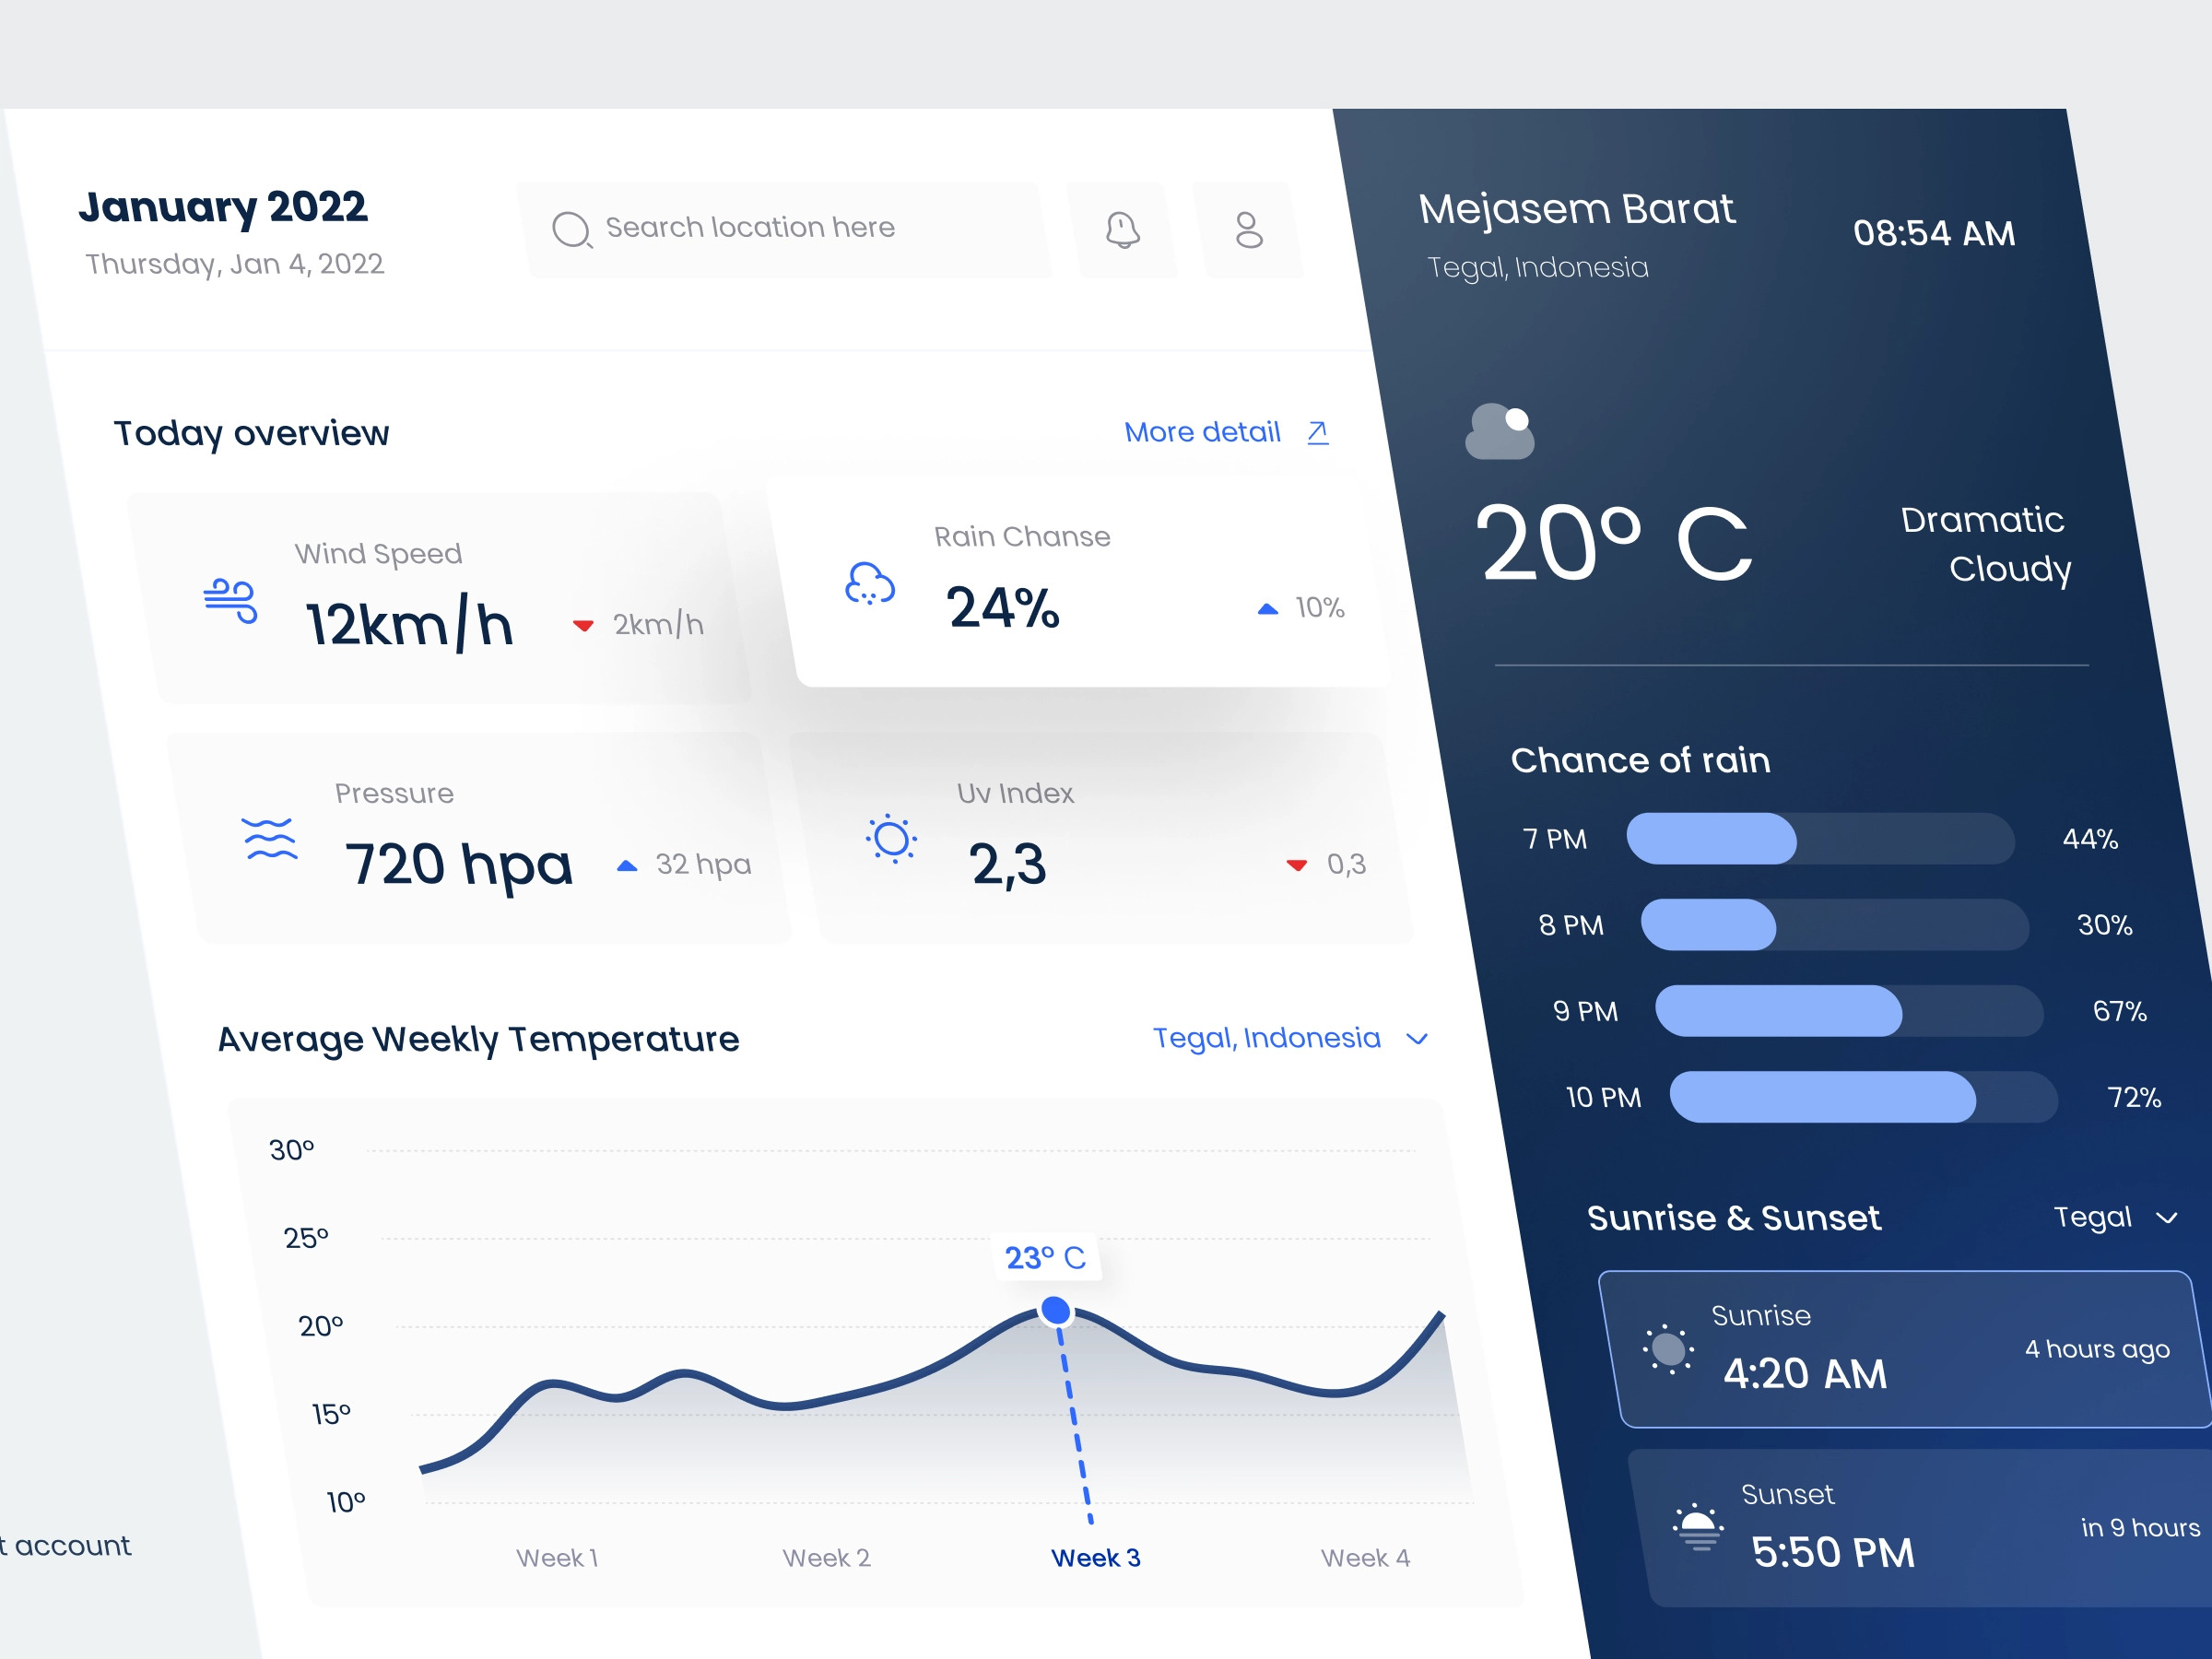
\includegraphics[width=.8\textwidth]{images/website/inspiration.jpg}
    \caption{Website reference design}
\end{figure}

\begin{figure}[H]
    \centering
    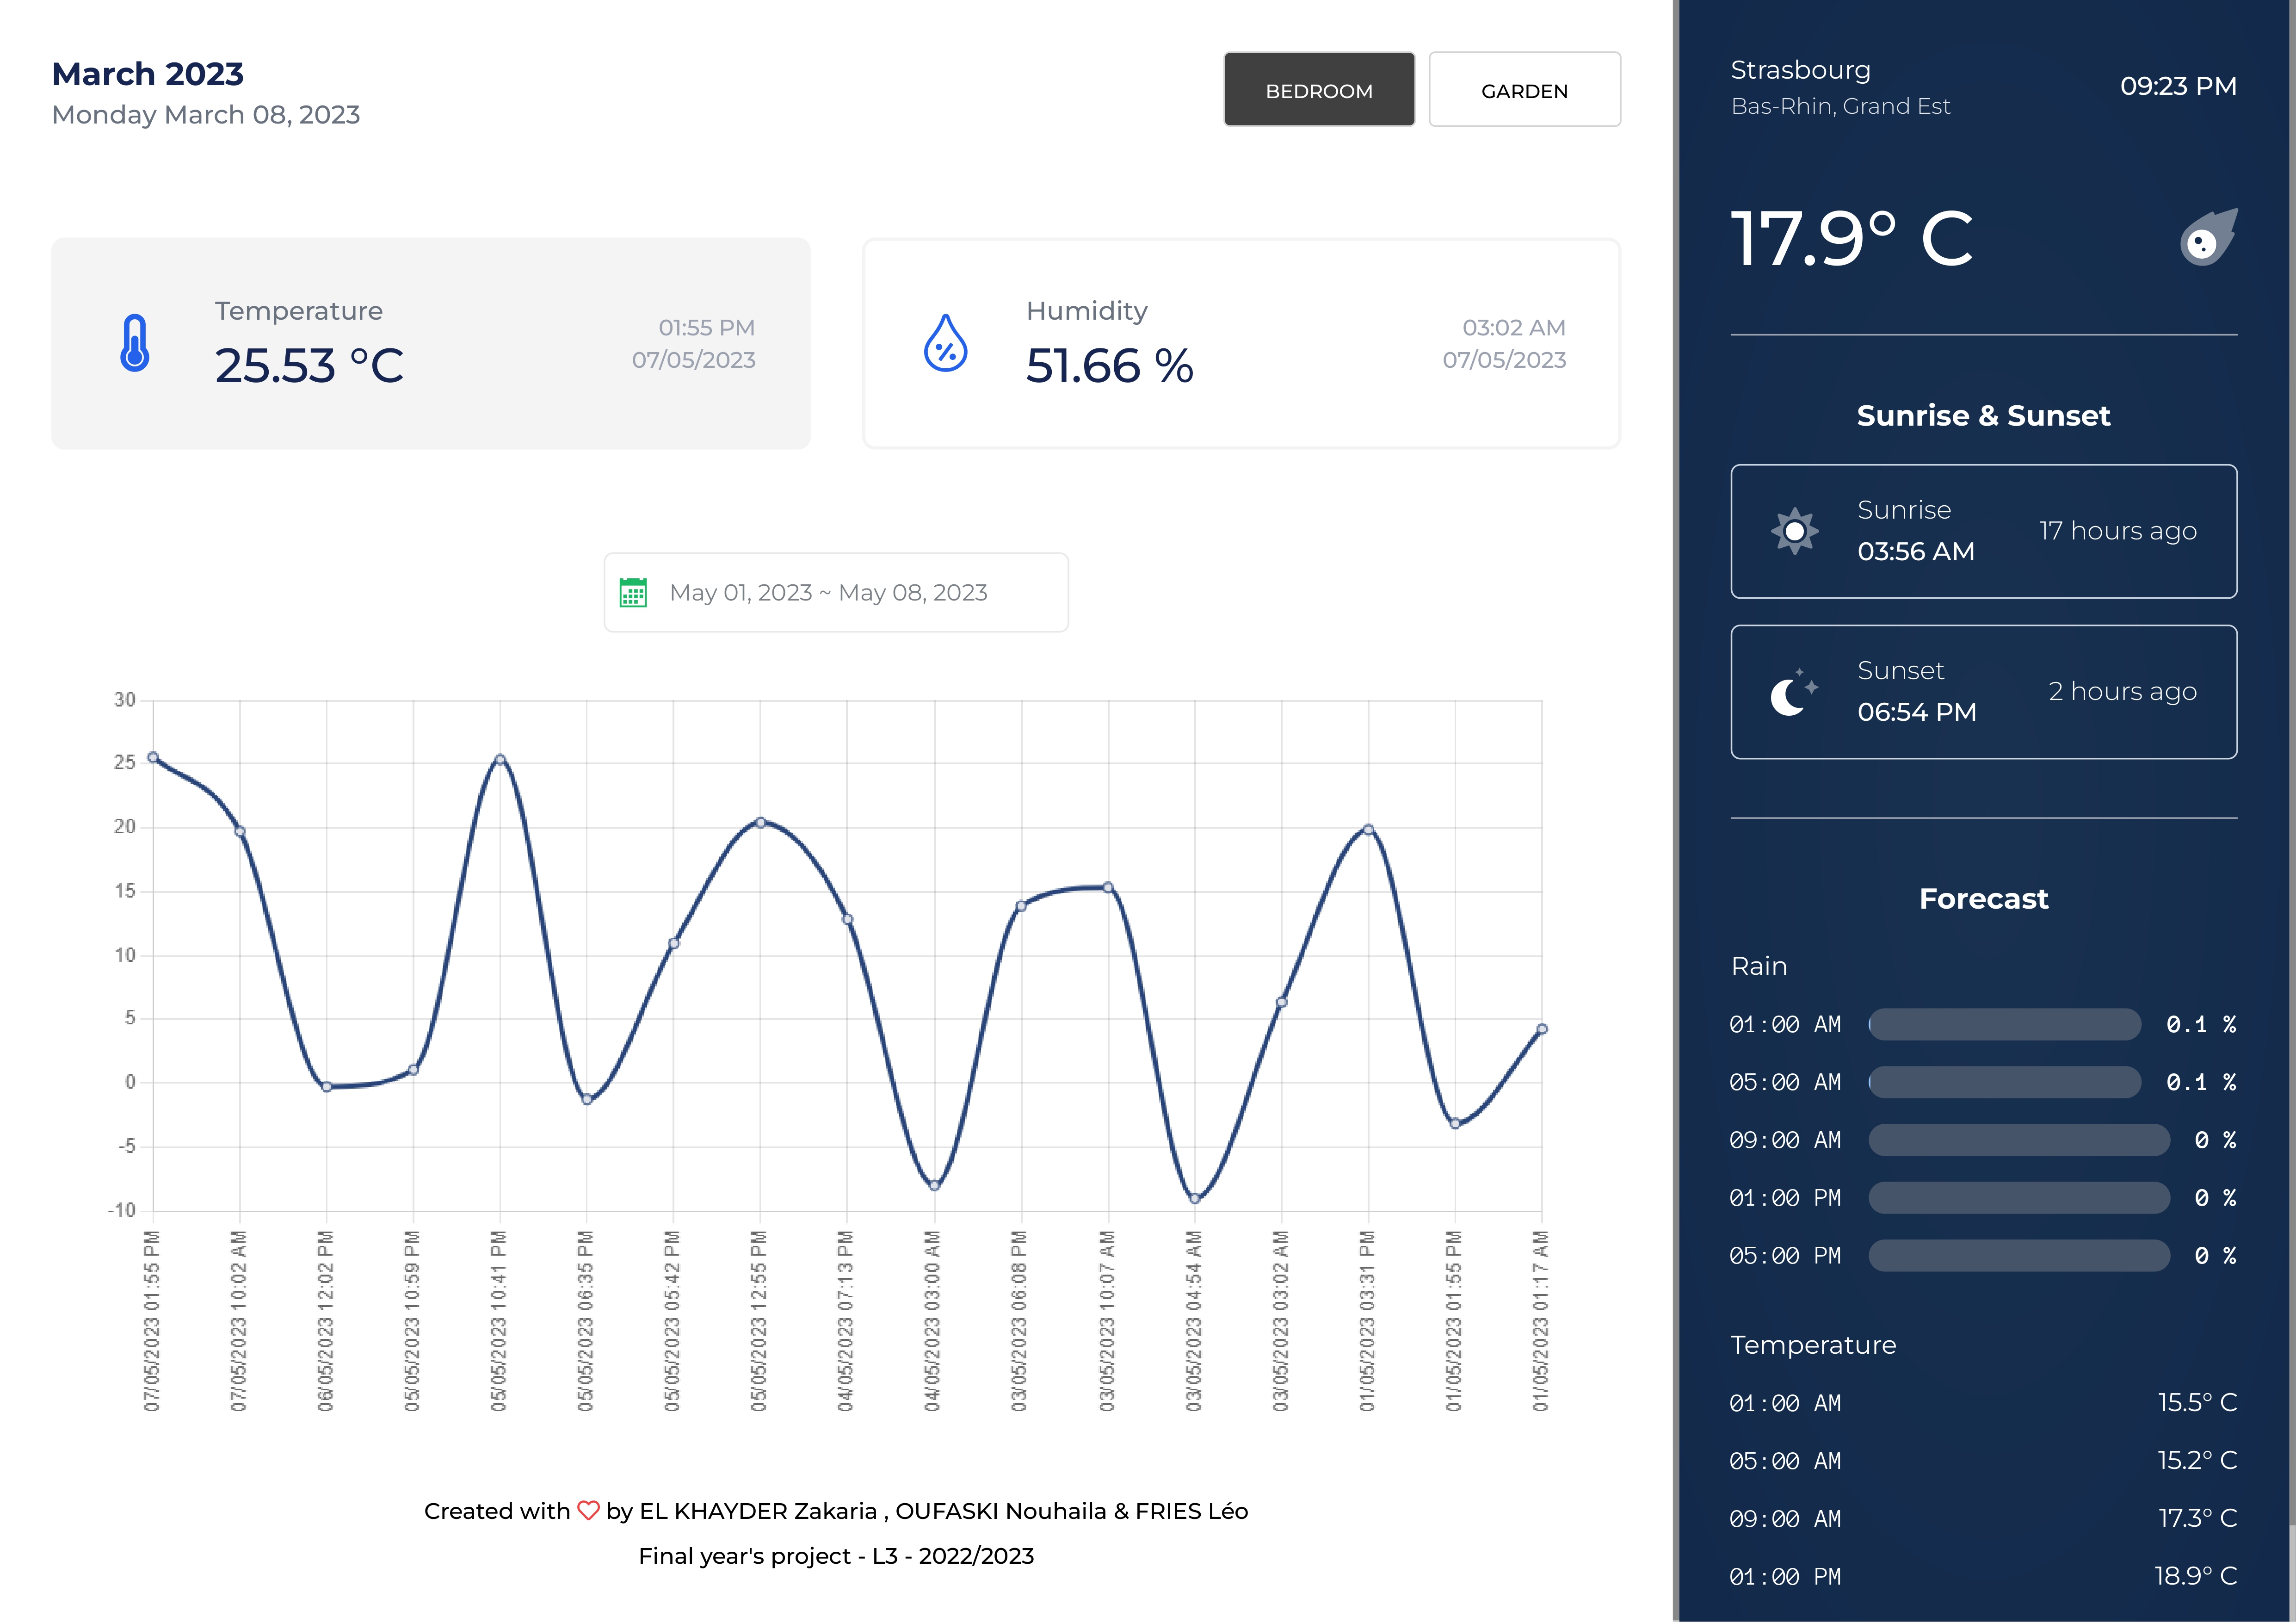
\includegraphics[width=\textwidth]{images/website/final_design.jpg}
    \caption{Website final result}
\end{figure}

\subsection{Functionalities}

\subsubsection{Geolocation}
We can get the user's current GPS location using the navigator's geolocation API, we can then reverse it back into an address using \href{https://geocode.maps.co}{geocode.maps.co} free API.

\subsubsection{Weather}
Using \href{https://open-meteo.com}{open-meteo.com} free API, we can get the current temperature for specific GPS coordinates.

\subsubsection{Sunrise \& sunset}
Using \href{https://sunrise-sunset.org}{sunrise-sunset.org} free API, we can get the sunrise \& sunset for specific GPS coordinates.

\subsubsection{Weather Forecast}
We can use \href{https://open-meteo.com}{open-meteo.com} free API to also get a weather forecast for specific GPS coordinates, such as rain probability and temperature forecast.

\subsubsection{Nodes data visualization}
We can parse the DB file that we can fetch from \verb|/api/db| and transform it into an object that we can use to analyze and visualize the data. \\
We used a graph to show different measurements of different nodes for a specific period that can be chosen with the date range selector. \\
We are also showing the latest measurement in hindsight for ease of use.
\section{Casing \& Protection}
We decided to think about the protection of the components of the nodes and of the central so we started to design different types of boxes on Autodesk Inventor with the intention of 3D printing it.

\subsection{Central Box}
First, we created the frame for the central, it should protect the borders of the screen and the components in a way to improve their lifespan and to give a better design to the central.
\begin{figure}[H]
    \centering
    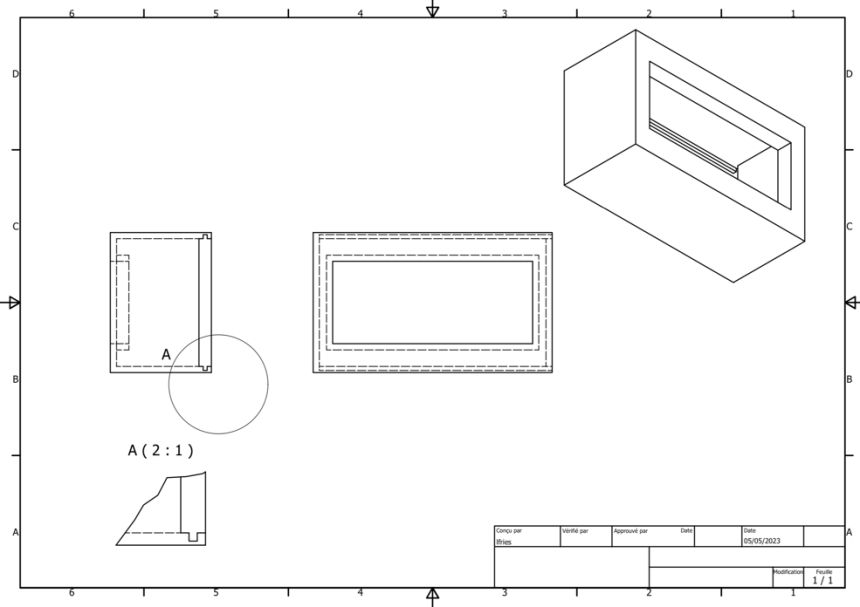
\includegraphics[width=.8\textwidth]{images/casing/img16.jpg}
    \caption{Plan of the frame for the screen}
\end{figure}

--- Step-by-Step Construction

First, we draw a rectangle with another rectangle hole in the middle of the first one. This hole will receive the screen of the central. We give the external rectangle a thickness of 3mm and then we create the walls of the box, they will have the same thickness as the first rectangle.

\begin{figure}[H]
    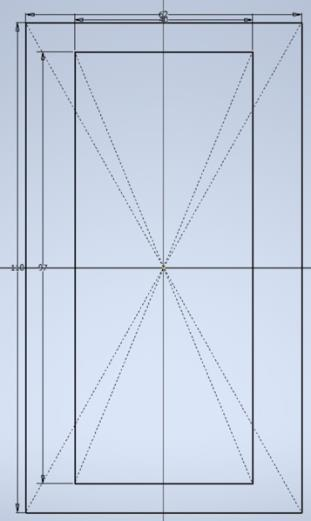
\includegraphics[height=7.5cm]{images/casing/img17.jpg}
    \hfill
    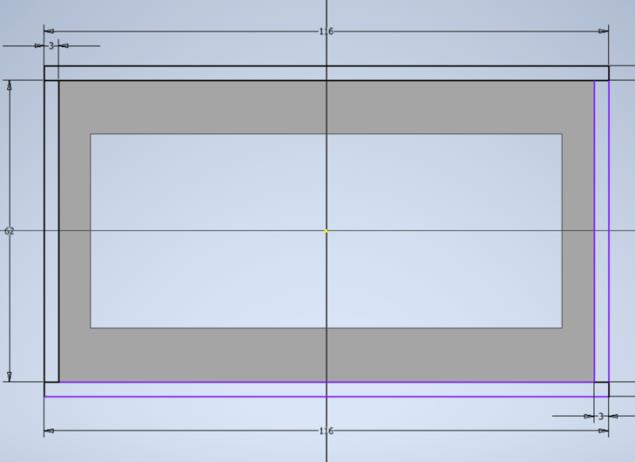
\includegraphics[height=7.5cm]{images/casing/img18.jpg}
\end{figure}

This box has to be high enough to contain all the components of the central so we decided to make it approximately 40mm high.
\begin{figure}[H]
    \centering
    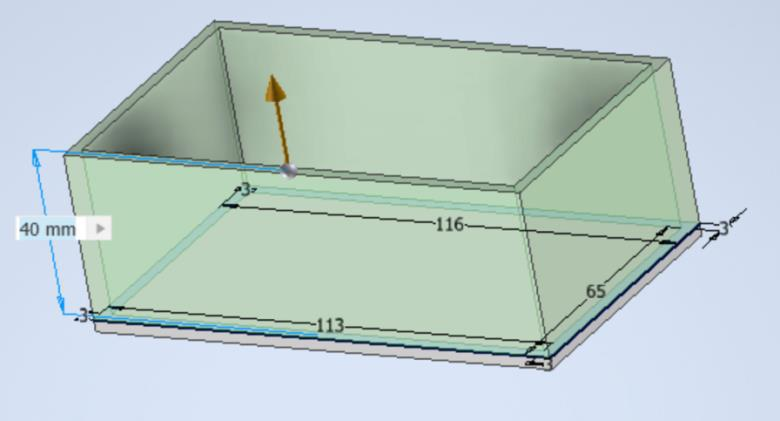
\includegraphics[width=.7\textwidth]{images/casing/img21.jpg}
\end{figure}

We also decided to integrate the screen as cleanly as possible, so we had to create elevations around the screen hole to put the screen at the same level as the front wall of the box. This way, the screen will be better protected and it will have a nicer design.
\begin{figure}[H]
    \centering
    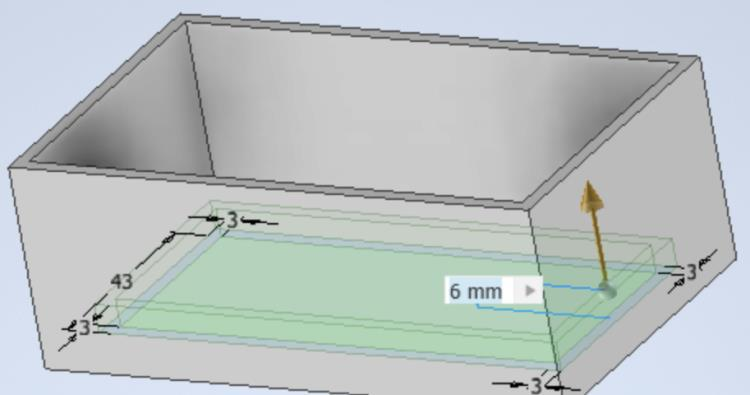
\includegraphics[width=.7\textwidth]{images/casing/img22.jpg}
\end{figure}

The last question about this box was "How to close it ?", to answer this question we decided to create a cover that would slide just behind the box and will remain tightly closed as we have left a fairly tight space.
\begin{figure}[H]
    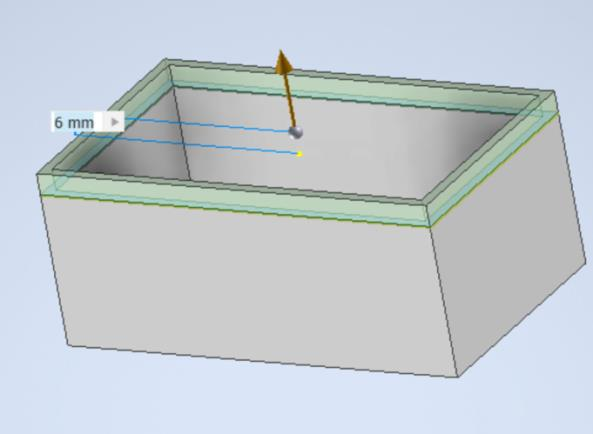
\includegraphics[height=6cm]{images/casing/img23.jpg}
    \hfill
    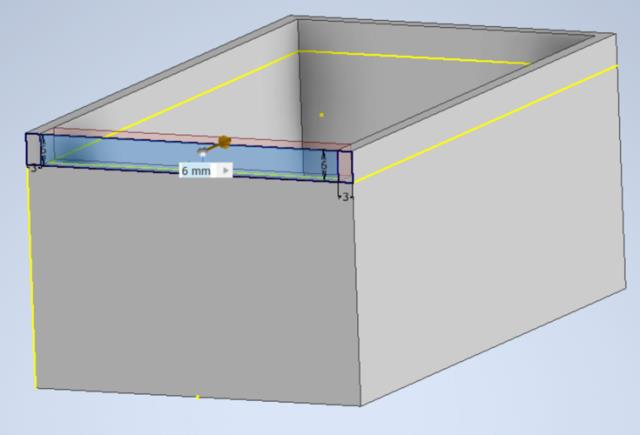
\includegraphics[height=6cm]{images/casing/img24.jpg}
\end{figure}

To let enough space for the cover and for the components, we had to enlarge a bit the box and to create an opening on one side. Finally, we had to create slits on both sides of the box to let the cover slide in its space.
\begin{figure}[H]
    \centering
    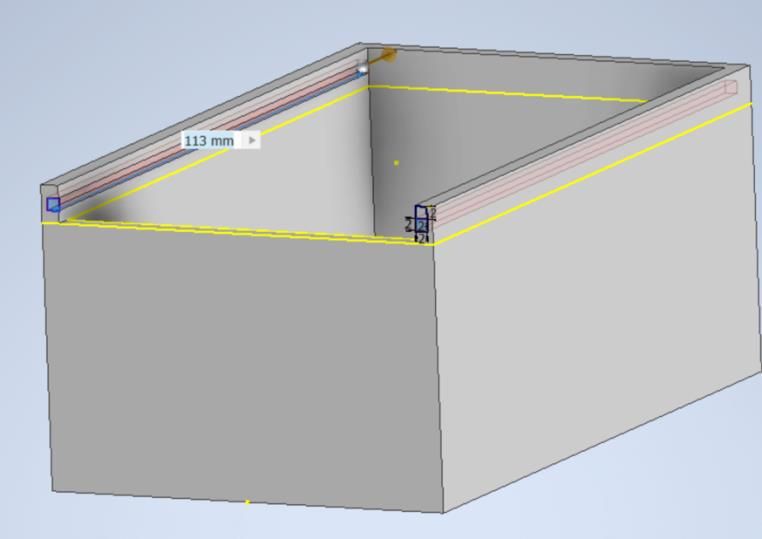
\includegraphics[width=.7\textwidth]{images/casing/img27.jpg}
\end{figure}

When we finished the design of the box we had to think about the design of the cover. We decided to create a simple board that could slip in and out of its space.
\begin{figure}[H]
    \centering
    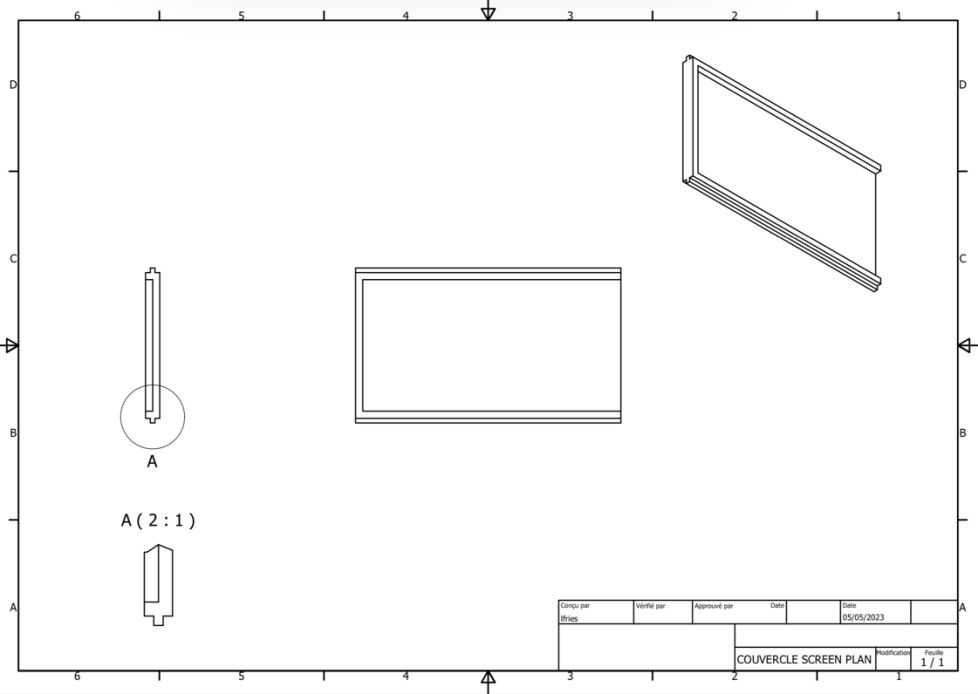
\includegraphics[width=.7\textwidth]{images/casing/img28.jpg}
    \caption{Plan of the cover of the central}
\end{figure}

To make this cover, we first started to create a rectangle of the right dimensions and we gave this rectangle a thickness of 3 mm. Then, we also added 3 mm to the sides of this rectangle so it can correctly close the box.
\begin{figure}[H]
    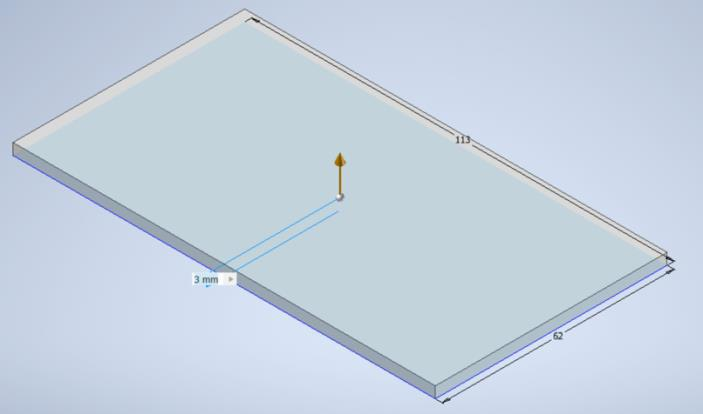
\includegraphics[height=5cm]{images/casing/img31.jpg}
    \hfill
    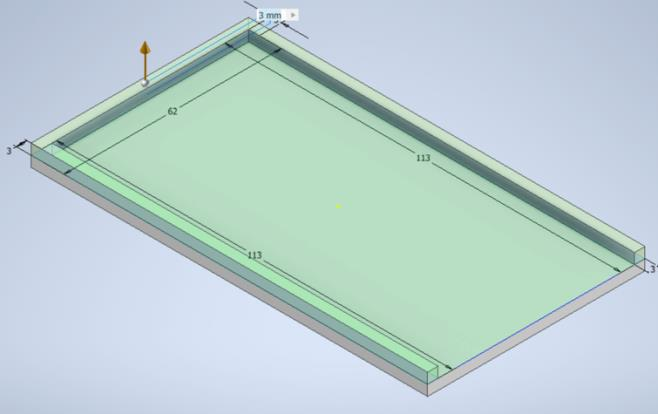
\includegraphics[height=5cm]{images/casing/img32.jpg}
\end{figure}

To finish, we created the male version of the slits in the box to allow the cover only to translate in one direction
\begin{figure}[H]
    \centering
    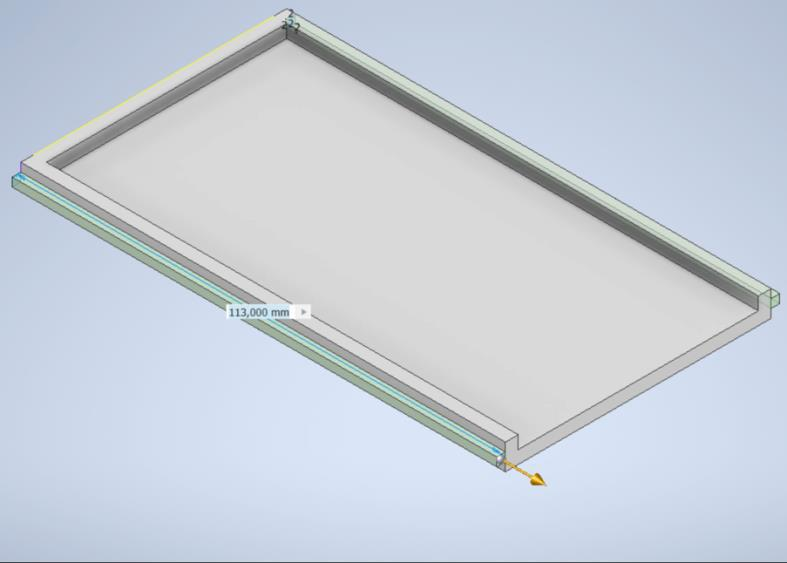
\includegraphics[width=.7\textwidth]{images/casing/img33.jpg}
\end{figure}

\subsection{Nodes Box}
To start with this box, we first created the frame that will receive the components as the Arduino Nano and the sensors. We have to let an opening on the front face of this box to let air pass through it and allow the sensors to get the right values. We also have to let an available place outside the box to place the antenna.
\begin{figure}[H]
    \centering
    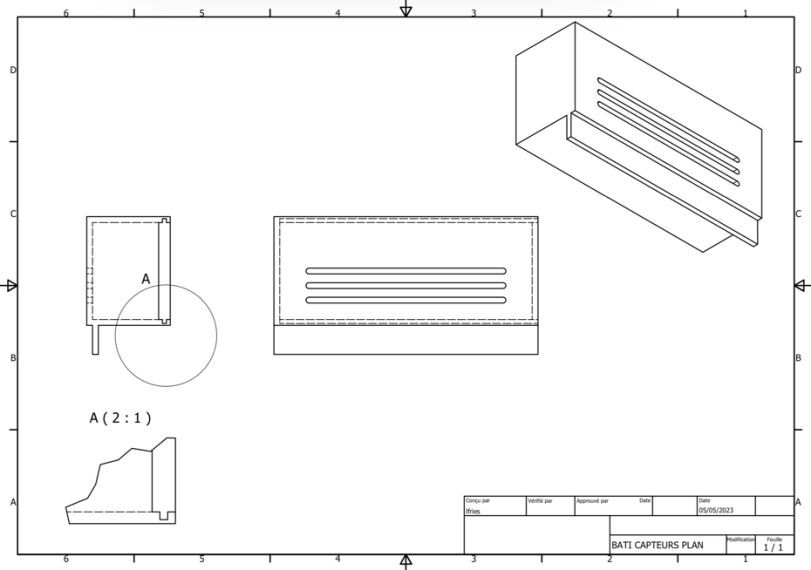
\includegraphics[width=.8\textwidth]{images/casing/img36.jpg}
    \caption{Plan of the box for the node}
\end{figure}

As for the central box, we created a rectangle of the right dimensions to receive the different parts to protect. We gave this rectangle a thickness of 3mm and also created walls to close the sides of the box.
\begin{figure}[H]
    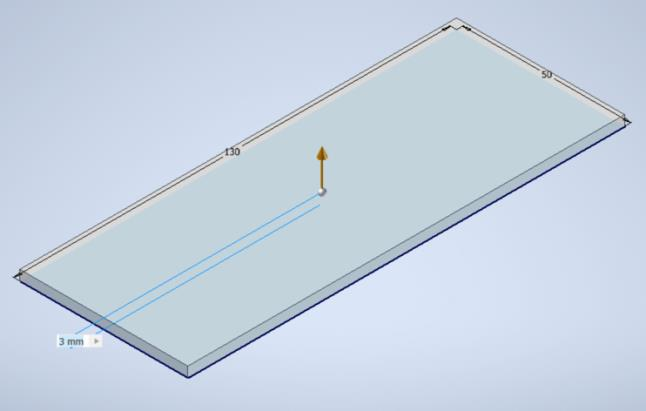
\includegraphics[height=5.5cm]{images/casing/img37.jpg}
    \hfill
    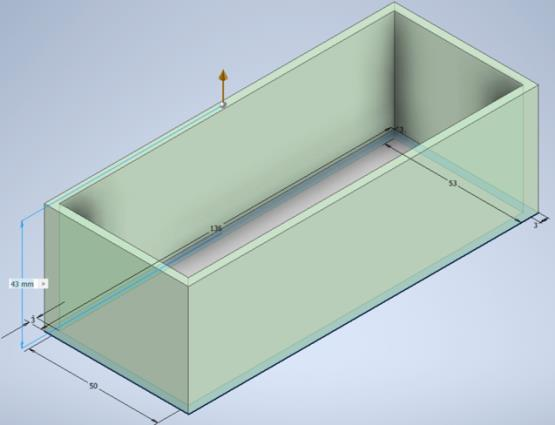
\includegraphics[height=5.5cm]{images/casing/img38.jpg}
\end{figure}

We also created the same slits as the first on the back of this box, in the way to close it with the same type of cover.
\begin{figure}[H]
    \centering
    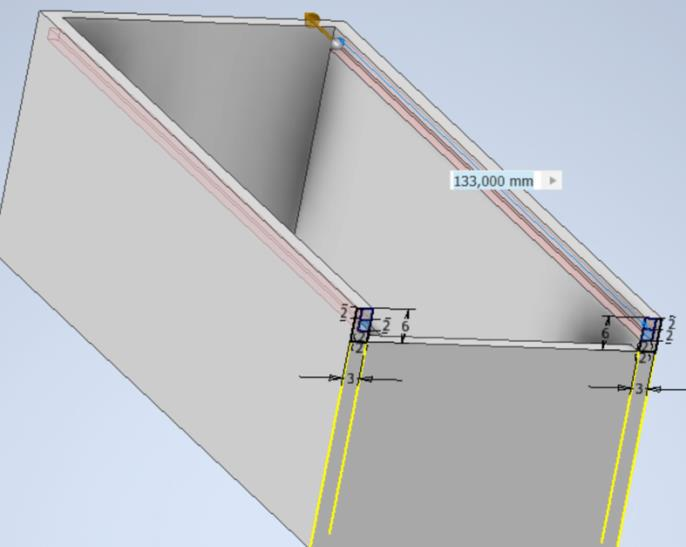
\includegraphics[width=.7\textwidth]{images/casing/img41.jpg}
\end{figure}

Finally, we had to create the openings on the front face and prepare space for the antenna.
\begin{figure}[H]
    \centering
    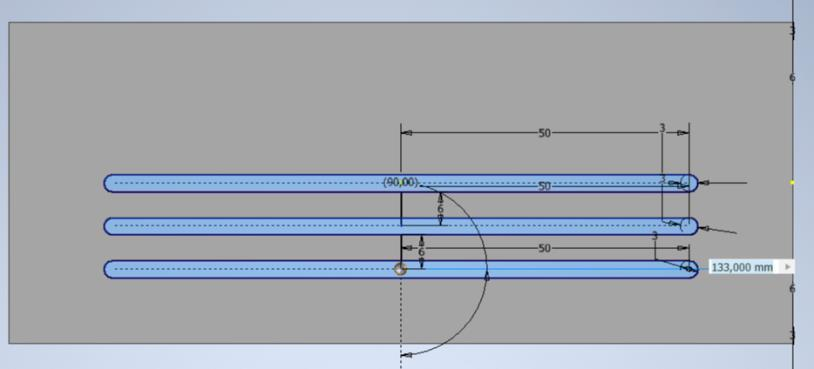
\includegraphics[width=.7\textwidth]{images/casing/img42.jpg}
    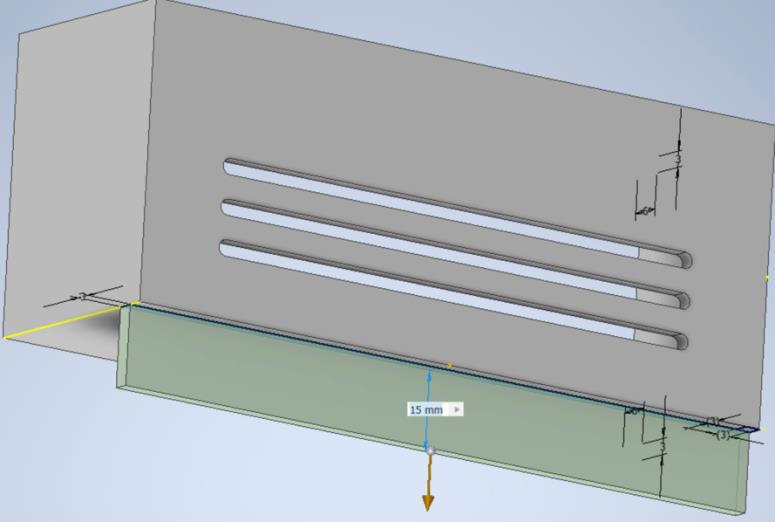
\includegraphics[width=.7\textwidth]{images/casing/img43.jpg}
\end{figure}

To close this box we created the same type of cover as for the first box.
\begin{figure}[H]
    \centering
    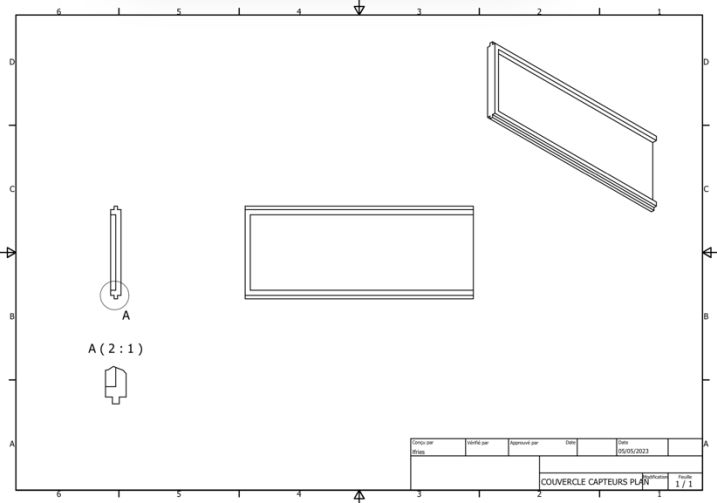
\includegraphics[width=.7\textwidth]{images/casing/img46.jpg}
    \caption{Plan of the cover for the node box}
\end{figure}

\subsection{Remarks}
After the impression and thinking of other problems, like putting the node box outside, we thought about different things that we could have done in another way. \\
--- First, we could have created a little roof on the front face of the node box, so in rainy situations, water wouldn’t really go inside it. \\
--- We also thought that it would have been better if we printed this box in white because, in the case of high temperatures outside, our black box will be hot really fast. \\
--- For both of the boxes, we also tough that we could have created a wall bracket to place our box on the wall with a screw or double-face adhesive.

\section{Conclusion}
In conclusion, the development and implementation of our weather station project have proven to be a
resounding success. Through the careful selection and integration of sensors, namely temperature, pressure,
and wind, we have been able to gather accurate and comprehensive weather data. The use of Arduino Nano
devices, strategically positioned in different locations, ensures reliable and consistent data collection from
different spots. \\
The adoption of LoRa communication has allowed for the seamless transmission of the collected information to the
central system, where it is processed and stored for future analysis. This central enables easy access to 
weather data through our website interface.
Overall, this project serves as a testament to our team's dedication, technical skills, and problem-solving abilities. \\
It has provided us with valuable hands-on experience in designing and implementing an effective project resulting
a well-functioning weather station.


\cleardoublepage
% Glossaries & acronyms
\pagenumbering{Roman}
\setcounter{page}{\theromancounter}

\printglossaries
\addcontentsline{toc}{section}{Glossary}

\end{document}
